% MAT670 -- Interlude H: Dynkin diagrams everywhere.
% Entirely new material (not in the handwritten notes). Labels prefixed DYN:.
% Placed at the very end of the book. All numerical claims checked with python3
% (Gram determinants, alcove vertices, hole counts, cell volumes, group orders).

\tikzset{
  DYNv/.style={circle,draw,fill=white,inner sep=0pt,minimum size=6.5pt},
  DYNa/.style={circle,draw,fill=black,inner sep=0pt,minimum size=6.5pt},
  DYNx/.style={circle,draw=flagcol,thick,fill=flagcol!35,inner sep=0pt,minimum size=7.5pt},
  DYNm/.style={font=\scriptsize,addcol},
  DYNl/.style={font=\scriptsize},
}

\chapter[Interlude H: Dynkin diagrams everywhere]{Interlude H: Dynkin diagrams everywhere}
\label{DYN:ch}

\begin{addedblock}
This interlude is new: it is not in the handwritten notes. It collects the places where the Dynkin
diagrams of Lectures~4--6 turn up again, in these notes and outside them, and asks in each place what
the diagram lets us read off. To keep it readable it is set in black; all of it should be read as
added material.
\end{addedblock}

Lecture~5 drew Dynkin diagrams in order to \emph{classify} root systems. Once the list was on the
board, the diagrams had done their job. But they kept coming back. Interlude~A found them inside
matrix algebras, Interlude~C folded them into quasicrystals, Interlude~D turned them into braid groups.
This last interlude takes the diagrams as the main characters and asks a few concrete questions about
objects we already know.
\begin{itemize}[nosep]
\item The inequality $\frac1p+\frac1q+\frac1r>1$ that ended the classification in Lecture~5: is it the
  same inequality that lists the Platonic solids?
\item Interlude~E proved that the icosahedron is not made of regular tetrahedra. Can the diagram of
  the icosahedron see that?
\item The FCC lattice has octahedral and tetrahedral holes, a cubic and a tetrahedral description,
  and the cuboctahedron as its kissing configuration. Which of these are visible on the diagram
  \tikz[baseline=-3pt]{\node[DYNv] (a) at (0,0) {}; \node[DYNv] (b) at (0.45,0) {}; \node[DYNv] (c) at (0.9,0) {};
  \draw (a)--(b)--(c);}\,?
\item Lecture~6 built $E_8$ by filling the deep holes of $D_8$. Can we \emph{see} the holes of $E_8$
  itself?
\end{itemize}
The answers are all yes, and most of them come from one extra node: the extended diagram of
Interlude~A (Section~\ref{LIE:sec:readoff}, item~7). At the end we tour the other places where the
ADE list appears (singularities, quivers, conformal field theory, subfactors, cubic surfaces), and
record in each case what the diagram says there.

Throughout, simply laced root systems are normalized with roots of norm $\ip\alpha\alpha=2$, so that
the Cartan matrix $C$ is the Gram matrix of the simple roots. We use the labelling of $E_8$ from
Lecture~6 (Section~\ref{L04b:sec:E8}): $\alpha_1,\dots,\alpha_6$ is a chain, $\alpha_7=e_6+e_7$ is
attached to $\alpha_5$, and $\alpha_8=-\frac12(1,\dots,1)$ is attached to $\alpha_7$.

%======================================================================
\section{One inequality, three times}
\label{DYN:sec:pqr}

\subsection*{The branch point, as a determinant}
Recall the last step of the classification (Section~\ref{L04b:sec:coxeter-cont}). A diagram with one
branch point has a centre $x$ and three arms of $p-1$, $q-1$, $r-1$ nodes. Call it $T_{p,q,r}$
(Figure~\ref{DYN:fig:Tpqr}); it has $p+q+r-2$ nodes. The lecture projected $x$ onto the span of the
arms and found that the diagram is admissible exactly when
$\frac1p+\frac1q+\frac1r>1$. The same computation, done with the Cartan matrix, gives an exact formula.

\begin{proposition}\label{DYN:prop:detT}
The Cartan matrix of $T_{p,q,r}$ (all edges simple, roots of norm $2$) has determinant
\[
  \det C(T_{p,q,r})=pqr\Big(\frac1p+\frac1q+\frac1r-1\Big).
\]
In particular $C(T_{p,q,r})$ is positive definite if and only if $\frac1p+\frac1q+\frac1r>1$.
\end{proposition}

\begin{proof}
Order the nodes with the centre first. Then
$C=\left(\begin{smallmatrix}2&b^T\\ b&C'\end{smallmatrix}\right)$, where
$C'=C(A_{p-1})\oplus C(A_{q-1})\oplus C(A_{r-1})$ is the Cartan matrix of the three arms and $b$ has an
entry $-1$ at the three arm nodes next to the centre. The Schur complement formula gives
\[
  \det C=\det C'\cdot\big(2-b^TC'^{-1}b\big).
\]
Two facts about the chain $A_k$ finish the job: $\det C(A_k)=k+1$ (expand along the last row:
$d_k=2d_{k-1}-d_{k-2}$), and the corner entry of $C(A_k)^{-1}$ is
$d_{k-1}/d_k=k/(k+1)$. Hence
\[
  \det C=pqr\Big(2-\frac{p-1}p-\frac{q-1}q-\frac{r-1}r\Big)=pqr\Big(\frac1p+\frac1q+\frac1r-1\Big).
\]
Since $C'$ is positive definite, $C$ is positive definite exactly when the Schur complement is
positive.
\end{proof}

The three terms $\frac{p-1}p$ are, up to the factor $2$ from our normalization, the squared
projections $\frac12(1-\frac1p)$ of the lecture. So the proof of Lecture~5 \emph{was} a Schur complement.
The formula is more than a test of positivity, though. Plugging in:
{\small\setlength{\arraycolsep}{4pt}\[
  \begin{array}{l|cccccccc}
  (p,q,r) & (1,q,r) & (2,2,n) & (2,3,3) & (2,3,4) & (2,3,5) & \begin{smallmatrix}(3,3,3),(2,4,4),\\(2,3,6)\end{smallmatrix} & (2,3,7)\\ \hline
  T_{p,q,r} & A_{q+r-1} & D_{n+2} & E_6 & E_7 & E_8 & \tilde E_6,\ \tilde E_7,\ \tilde E_8 & E_{10}\\
  \det C & q+r & 4 & 3 & 2 & 1 & 0 & -1
  \end{array}
\]}
These are the determinants $\det C$ that Interlude~A used to read off the packing densities of the
root lattices, now all from one formula. On the $E$-series $E_n=T_{2,3,n-3}$ the formula is linear:
\begin{equation}\label{DYN:eq:Edet}
  \det C(E_n)=6(n-3)\Big(\frac1{n-3}-\frac16\Big)=9-n .
\end{equation}
At $n=9$ the determinant vanishes. $E_9=T_{2,3,6}$ is the extended diagram $\tilde E_8$, the
diagram of the affine Weyl group that tiles $\R^8$ by alcoves (Section~\ref{LIE:sec:torus}). At
$n=10$ the form becomes indefinite, of signature $(9,1)$. The determinant $-1$ says the $E_{10}$ lattice is
unimodular; it is the even unimodular Lorentzian lattice $\mathrm{II}_{9,1}$.

\begin{figure}[ht]
\centering
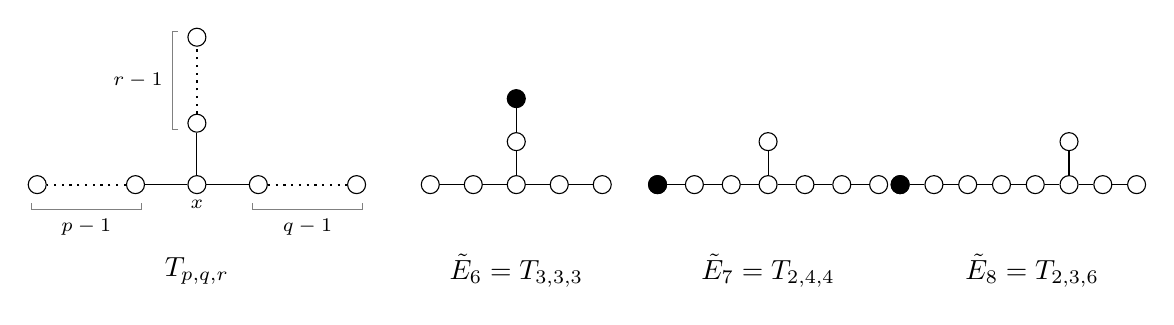
\begin{tikzpicture}[scale=0.78]
  \begin{scope}
    \node[DYNv] (x) at (0,0) {}; \node[DYNl,below=2pt] at (0,0) {$x$};
    \node[DYNv] (u1) at (-1,0) {}; \node[DYNv] (u2) at (-2.6,0) {};
    \node[DYNv] (v1) at (1,0) {}; \node[DYNv] (v2) at (2.6,0) {};
    \node[DYNv] (w1) at (0,1) {}; \node[DYNv] (w2) at (0,2.4) {};
    \draw (u1)--(x)--(v1); \draw (x)--(w1);
    \draw[dotted,thick] (u1)--(u2); \draw[dotted,thick] (v1)--(v2); \draw[dotted,thick] (w1)--(w2);
    \draw[gray] (-2.7,-0.3)--(-2.7,-0.4)--(-0.9,-0.4)--(-0.9,-0.3); \node[DYNl,below] at (-1.8,-0.4) {$p-1$};
    \draw[gray] (0.9,-0.3)--(0.9,-0.4)--(2.7,-0.4)--(2.7,-0.3); \node[DYNl,below] at (1.8,-0.4) {$q-1$};
    \draw[gray] (-0.3,0.9)--(-0.4,0.9)--(-0.4,2.5)--(-0.3,2.5); \node[DYNl,left] at (-0.4,1.7) {$r-1$};
    \node at (0,-1.4) {$T_{p,q,r}$};
  \end{scope}
  % E6~ = T333
  \begin{scope}[xshift=5.2cm]
    \foreach \i in {-2,...,2} \node[DYNv] (a\i) at (0.7*\i,0) {};
    \node[DYNv] (b1) at (0,0.7) {}; \node[DYNa] (b2) at (0,1.4) {};
    \foreach \i [evaluate=\i as \j using int(\i+1)] in {-2,...,1} \draw (a\i)--(a\j);
    \draw (a0)--(b1)--(b2);
    \node at (0,-1.4) {$\tilde E_6=T_{3,3,3}$};
  \end{scope}
  % E7~ = T244
  \begin{scope}[xshift=9.3cm]
    \foreach \i in {-3,...,3} \node[DYNv] (a\i) at (0.6*\i,0) {};
    \node[DYNa] (a-3) at (-1.8,0) {};
    \node[DYNv] (b1) at (0,0.7) {};
    \foreach \i [evaluate=\i as \j using int(\i+1)] in {-3,...,2} \draw (a\i)--(a\j);
    \draw (a0)--(b1);
    \node at (0,-1.4) {$\tilde E_7=T_{2,4,4}$};
  \end{scope}
  % E8~ = T236
  \begin{scope}[xshift=14.2cm]
    \foreach \i in {-5,...,2} \node[DYNv] (a\i) at (0.55*\i,0) {};
    \node[DYNa] (a-5) at (-2.75,0) {};
    \node[DYNv] (b1) at (0,0.7) {};
    \foreach \i [evaluate=\i as \j using int(\i+1)] in {-5,...,1} \draw (a\i)--(a\j);
    \draw (a0)--(b1);
    \node at (-0.6,-1.4) {$\tilde E_8=T_{2,3,6}$};
  \end{scope}
\end{tikzpicture}
\caption{The diagram $T_{p,q,r}$, with arms of $p-1$, $q-1$, $r-1$ nodes, and the three cases with
$\frac1p+\frac1q+\frac1r=1$. These are the extended diagrams $\tilde E_6,\tilde E_7,\tilde E_8$; the
black node is the extra (affine) node.}
\label{DYN:fig:Tpqr}
\end{figure}

\subsection*{Triangles on the sphere}
Now forget Dynkin diagrams and draw a triangle on the unit sphere with angles $\frac\pi p$, $\frac\pi q$,
$\frac\pi r$. By Gauss--Bonnet its area is the angle excess,
\[
  \operatorname{area}=\pi\Big(\frac1p+\frac1q+\frac1r-1\Big),
\]
so the triangle exists on the sphere exactly when $\frac1p+\frac1q+\frac1r>1$. It exists in the
Euclidean plane when the sum equals $1$, and in the hyperbolic plane when it is less than $1$. The
reflections in its three sides generate a group that tiles the sphere by copies of the triangle. There
are $4\pi/\operatorname{area}$ copies, and the rotations (products of two reflections) form a subgroup
of index $2$:
\[
  \abs{G^+_{p,q,r}}=\frac{2}{\frac1p+\frac1q+\frac1r-1}.
\]
For $(2,3,3)$, $(2,3,4)$, $(2,3,5)$ this gives $12$, $24$, $60$: the rotation groups of the tetrahedron,
the cube (or octahedron), and the icosahedron (or dodecahedron). For $(2,2,n)$ it gives the dihedral
group of order $2n$, the symmetries of a regular $n$-gon viewed as a flat polyhedron (a ``dihedron'').
The integers $p,q,r$ are the orders of the rotation axes: for the icosahedron, $2$ through the edge
midpoints, $3$ through the face centres and $5$ through the vertices. The Euclidean cases $(3,3,3)$,
$(2,4,4)$, $(2,3,6)$ are the reflection groups of the equilateral triangle, the isosceles right
triangle and the $30$--$60$--$90$ triangle, the kaleidoscopes of the hexagonal and square lattices.

Comparing with Proposition~\ref{DYN:prop:detT} we get a curious identity:
\[
  \det C(T_{p,q,r})=\frac{2pqr}{\abs{G^+_{p,q,r}}}\qquad\text{e.g.}\quad
  \det C(E_8)=\frac{2\cdot30}{60}=1,\quad \det C(E_6)=\frac{2\cdot18}{12}=3.
\]
So \emph{the branch diagrams $D_n,E_6,E_7,E_8$ are the dihedra and the Platonic solids}. (The chains
$A_n=T_{1,q,r}$ do not fit this pattern on the nose; Section~\ref{DYN:sec:elsewhere} matches them with
the cyclic groups.) The arms of $E_8$ have lengths $1,2,4$ because the icosahedron
has rotations of orders $2,3,5$. So far this is a coincidence of numbers. Section~\ref{DYN:sec:elsewhere}
explains it: the resolution of the singularity $\C^2/\Gamma$, for $\Gamma$ the binary icosahedral group,
\emph{is} a $T_{2,3,5}$ of curves.

\subsection*{Coxeter's criterion}
There is a third appearance, which puts the first two in one frame. A \emph{Coxeter diagram} has a node for each
generator $s_i$ and an edge labelled $m_{ij}$ when $(s_is_j)^{m_{ij}}=1$ (unlabelled means $3$, no edge
means $2$). Its \emph{Schl\"afli} (or Gram) matrix is
\[
  G_{ij}=-\cos\frac{\pi}{m_{ij}},\qquad G_{ii}=1,
\]
the Gram matrix of unit normals to mirrors meeting at angles $\pi/m_{ij}$. For a crystallographic
diagram, $G$ is the Cartan matrix rescaled ($G=\frac12C$ in the simply laced case).

\begin{theorem}[Coxeter 1934]\label{DYN:thm:coxeter}
Let $\Gamma$ be a connected Coxeter diagram with Schl\"afli matrix $G$. The group
$\langle s_i\mid s_i^2,(s_is_j)^{m_{ij}}\rangle$ is a finite reflection group if and only if $G$ is
positive definite. It acts as a discrete group generated by reflections of a Euclidean space, with a
simplex as fundamental domain, if and only if $G$ is positive semidefinite with a one-dimensional kernel.
The connected positive definite diagrams are $A_n,B_n,D_n,E_6,E_7,E_8,F_4,G_2$, together with the
non-crystallographic $H_3$, $H_4$ and $I_2(m)$.
\end{theorem}

For three mirrors forming a triangle $(p,q,r)$,
$\det G=1-a^2-b^2-c^2-2abc$ with $a=\cos\frac\pi p$, $b=\cos\frac\pi q$, $c=\cos\frac\pi r$. We checked
numerically that this is positive, zero, negative in the spherical, Euclidean, hyperbolic cases
(for example $\det G=0.0955$ for $(2,3,5)$ and $-0.0617$ for $(2,3,7)$). A Platonic solid $\{p,q\}$ has
the linear diagram $\circ\overset{p}{\text{---}}\circ\overset{q}{\text{---}}\circ$, whose determinant is
$1-\cos^2\frac\pi p-\cos^2\frac\pi q$. It is positive if and only if
$\frac1p+\frac1q>\frac12$, the classical condition for $\{p,q\}$ to exist. This is the triangle
$(2,p,q)$ again. So the classification of Platonic solids, of spherical triangle groups and of
branched Dynkin diagrams are three readings of one inequality.

%======================================================================
\section[The icosahedron, seen by Coxeter]{The icosahedron is not made of regular tetrahedra, seen by Coxeter}
\label{DYN:sec:icosa}

Interlude~E (Section~\ref{TET:sec}) proved, with a ring of six balls and the triangle inequality on
the sphere, that $20$ regular tetrahedra glued at a common vertex do not close up into an icosahedron.
Around each of the $12$ edges from the centre there would be $5$ tetrahedra, and $5$ dihedral angles
$\arccos\frac13\approx70.53^\circ$ leave a gap of $7.36^\circ$. Now look at the same configuration
through its Coxeter diagram.

A regular polytope or honeycomb with Schl\"afli symbol $\{p,q,r\}$ has the linear Coxeter diagram
\[
  \circ\overset{p}{\text{---}}\circ\overset{q}{\text{---}}\circ\overset{r}{\text{---}}\circ .
\]
The first three nodes generate the symmetry group of a cell $\{p,q\}$, the last three that of the vertex
figure $\{q,r\}$, and the label $r$ says that $r$ cells surround each edge. ``Twenty tetrahedra around a
vertex, forming an icosahedron'' is the local structure of $\{3,3,5\}$: cell a tetrahedron $\{3,3\}$,
vertex figure an icosahedron $\{3,5\}$, five cells around an edge.

\begin{proposition}\label{DYN:prop:gram335}
The Schl\"afli matrix of $\{p,q,r\}$ has determinant
\[
  \det G_{\{p,q,r\}}=\sin^2\frac\pi p\,\sin^2\frac\pi r-\cos^2\frac\pi q .
\]
For $\{3,3,r\}$ this is $\frac12-\frac34\cos^2\frac\pi r$, and
\[
  \det G_{\{3,3,r\}}\ \gtreqless\ 0\quad\iff\quad r\cdot\arccos\tfrac13\ \lesseqgtr\ 2\pi .
\]
The values are $\frac5{16}$, $\frac18$, $\frac{5-3\tau}{16}\approx0.0091$, $-\frac1{16}$ for
$r=3,4,5,6$, where $\tau=\frac{1+\sqrt5}2$.
\end{proposition}

\begin{proof}
For a tridiagonal matrix with $1$ on the diagonal and off-diagonal entries $-a,-b,-c$, the leading
minors satisfy $D_k=D_{k-1}-(\text{entry})^2D_{k-2}$. So $D_2=1-a^2$, $D_3=1-a^2-b^2$, and
\[
  D_4=D_3-c^2D_2=(1-a^2)(1-c^2)-b^2 .
\]
With $a=b=\frac12$ this is $\frac34(1-c^2)-\frac14=\frac12-\frac34c^2$. It vanishes if and only if
$c^2=\cos^2\frac\pi r=\frac23$, that is, if and only if $\cos\frac{2\pi}r=2c^2-1=\frac13$, that is,
$\frac{2\pi}r=\arccos\frac13$. As $r$ grows, $c^2$ grows, so the sign of $\det G$ is the sign of
$2\pi-r\arccos\frac13$. For $r=5$, $c=\cos\frac\pi5=\frac\tau2$ and $c^2=\frac{\tau+1}4$, which gives
$\frac12-\frac{3(\tau+1)}{16}=\frac{5-3\tau}{16}$.
\end{proof}

So the sign of a $4\times4$ determinant is exactly the sign of the gap left by $r$ regular tetrahedra
around an edge. The critical value is $r=2\pi/\arccos\frac13\approx5.104$, not an integer, so
there is no Euclidean honeycomb of regular tetrahedra (Figure~\ref{DYN:fig:gram}):
\begin{itemize}[nosep]
\item $r=3,4,5$: positive definite, spherical. These are the $5$-cell $\{3,3,3\}$, the $16$-cell
  $\{3,3,4\}$ and the $600$-cell $\{3,3,5\}$, with groups $A_4$, $B_4$, $H_4$.
\item $r=6$: indefinite, hyperbolic. Six tetrahedra around an edge overshoot, and $\{3,3,6\}$ is a
  honeycomb of hyperbolic space with ideal vertices.
\item Euclidean: never.
\end{itemize}
The icosahedral case $r=5$ is spherical, but only just: $(5-3\tau)/16\approx0.0091$, against
$\frac5{16}$ and $\frac18$ for $r=3,4$. This small number is the $7.36^\circ$ of Interlude~E. A flat
icosahedron of regular tetrahedra would need $\det G=0$. On the $3$-sphere the curvature closes the
gap, and $600$ regular spherical tetrahedra form the $600$-cell, the ``ideal'' icosahedral order of
Section~\ref{SM:sec:curved}. Its Schl\"afli determinant is positive, which says that $H_4$ is a finite
reflection group and that the tiling closes up on a sphere. In Schl\"afli's original form the criterion
reads $\sin\frac\pi p\sin\frac\pi r>\cos\frac\pi q$, and for $\{3,3,5\}$ it is
$0.5090>0.5$.

\begin{figure}[ht]
\centering
\begin{tikzpicture}[xscale=1.25,yscale=9]
  \draw[-{Stealth}] (2.6,0)--(8.3,0) node[right,DYNl]{$r$};
  \draw[-{Stealth}] (2.8,-0.15)--(2.8,0.37) node[above,DYNl]{$\det G_{\{3,3,r\}}$};
  \foreach \y in {-0.1,0.1,0.2,0.3} {\draw (2.75,\y)--(2.85,\y); \node[left,DYNl] at (2.75,\y) {$\y$};}
  \draw[thick,addcol,domain=2.9:7.7,samples=120] plot (\x,{0.5-0.75*cos(180/\x)^2});
  \foreach \r/\v in {3/0.3125,4/0.125,5/0.00912,6/-0.0625,7/-0.1088} {\fill (\r,\v) ellipse (0.05 and 0.007); \draw[gray!60] (\r,0)--(\r,-0.006); \node[below,DYNl] at (\r,-0.006) {$\r$};}
  \fill[flagcol] (5.104,0) ellipse (0.06 and 0.008);
  \draw[flagcol,-{Stealth}] (5.9,0.12)--(5.15,0.012);
  \node[flagcol,DYNl,align=left,anchor=west] at (5.9,0.135) {$r=2\pi/\arccos\frac13\approx5.104$\\Euclidean case, not an integer};
  \node[DYNl,anchor=west] at (3.1,0.32) {$5$-cell};
  \node[DYNl,anchor=south west] at (4.05,0.13) {$16$-cell};
  \node[DYNl,anchor=south east] at (4.92,0.012) {$600$-cell};
  \node[DYNl,anchor=south west] at (6.1,-0.055) {hyperbolic};
\end{tikzpicture}
\caption{The Schl\"afli determinant $\frac12-\frac34\cos^2\frac\pi r$ of $\{3,3,r\}$, with $r$ treated as
a real variable. It crosses zero where $r$ regular tetrahedra exactly fill the space around an edge.
The value at $r=5$ is positive but tiny.}
\label{DYN:fig:gram}
\end{figure}

\paragraph{Reading the $600$-cell off its diagram.} The diagram of $H_4$ also counts. By Wythoff's
construction the $k$-faces of $\{p,q,r\}$ correspond to cosets of the subgroup generated by all nodes
except the $(k+1)$-st, so their number is $\abs W$ divided by the order of that subgroup. With
$\abs{W(H_4)}=14400$ (Interlude~C):
\begin{gather*}
  \text{vertices: }\frac{14400}{\abs{W(H_3)}}=\frac{14400}{120}=120,\qquad
  \text{edges: }\frac{14400}{\abs{W(A_1)}\,\abs{W(I_2(5))}}=\frac{14400}{2\cdot10}=720,\\
  \text{triangles: }\frac{14400}{\abs{W(A_2)}\,\abs{W(A_1)}}=\frac{14400}{6\cdot2}=1200,\qquad
  \text{cells: }\frac{14400}{\abs{W(A_3)}}=\frac{14400}{24}=600 .
\end{gather*}
The vertex stabilizer is $H_3$, the symmetry group of the icosahedral vertex figure.

\subsection*{Why a lattice cannot do it}
The label $5$ is also what keeps icosahedral order out of crystals.

\begin{proposition}[Crystallographic restriction]\label{DYN:prop:cryst}
If a rotation of order $m$ maps a lattice $\Lat\subset\R^d$ to itself, then its characteristic
polynomial has integer coefficients. For $d=2,3$ this forces $m\in\{1,2,3,4,6\}$. More generally, a
lattice with a symmetry of order $5$ has dimension at least $4$. If a group isomorphic to the icosahedral
rotation group $A_5$ preserves a lattice in $\R^d$ and acts on some $3$-dimensional subspace as the
rotations of an icosahedron, then $d\ge6$.
\end{proposition}

\begin{proof}
In a basis of $\Lat$ the rotation is an integer matrix. For $d=2$ its trace $2\cos\frac{2\pi}m$ is an
integer, and for $d=3$ the trace $1+2\cos\frac{2\pi}m$ is; either way
$\cos\frac{2\pi}m\in\{0,\pm\frac12,\pm1\}$. An integer matrix of order $5$ has eigenvalues that are fifth
roots of unity, closed under Galois conjugation; a primitive one brings all four primitive ones with it,
so $d\ge4$. For the icosahedral group $A_5$, the two irreducible real representations of dimension $3$ have
characters involving $\sqrt5$ and are swapped by $\sqrt5\mapsto-\sqrt5$. The representation on
$\Lat\otimes\Q$ is rational, so if it contains one of them it contains the other equally often, and
$d\ge3+3$. (The condition on the $3$-dimensional subspace matters: $A_5\subset\Sigma_5=W(A_4)$ preserves the
$4$-dimensional lattice $A_4$, acting through its rational $4$-dimensional representation.)
\end{proof}

For a reflection group the rotation $s_is_j$ has order $m_{ij}$, so the proposition is the
crystallographic table of Lecture~4 again: $4\cos^2\frac\pi m\in\{0,1,2,3\}$ allows
$m\in\{2,3,4,6\}$, and $4\cos^2\frac\pi5=\tau+1$ is irrational. The bounds are attained. The Coxeter
element of $A_4$ has order $h=5$ (Interlude~A, item~3), and Interlude~C (Theorem~\ref{ERG:thm:fold})
realizes $H_3$ inside $D_6$ and $H_4$ inside $E_8$. That is the precise sense in which the $E_8$ lattice
``contains'' the icosahedral order that is impossible in a flat crystal: the $240$ roots project to two
$600$-cells. In three dimensions the best one can do is a quasicrystal.

%======================================================================
\section{The FCC lattice, read off its diagrams}
\label{DYN:sec:fcc}

The FCC lattice is the root lattice $A_3$, the densest packing in $\R^3$ (Hales). We now go through
its features one by one and find each on a diagram.

\subsection*{Two names: $A_3=D_3$}
Lectures~5 and~6 met FCC twice: as $A_3=\{x\in\Z^4:\sum x_i=0\}$ and, in the remark $D_3=A_3$ after the
classification, as $D_3=\{x\in\Z^3:x_1+x_2+x_3\text{ even}\}$.
The diagrams agree: $D_3$ would be a chain of two nodes both joined to a third, which is the chain
$A_3$. That is why Theorem~\ref{L04a:thm:classification} starts $D_n$ at $n=4$. An explicit isometry is
\[
  f(x)=\tfrac12\big(x_1+x_2-x_3-x_4,\ x_1-x_2+x_3-x_4,\ x_1-x_2-x_3+x_4\big).
\]
It sends $e_1,e_2,e_3,e_4$ to the four vertices $\frac12(1,1,1)$, $\frac12(1,-1,-1)$,
$\frac12(-1,1,-1)$, $\frac12(-1,-1,1)$ of a regular tetrahedron inscribed in the cube, and
$e_1-e_2\mapsto(0,1,1)$, $e_1-e_3\mapsto(1,0,1)$, and so on, so the $12$ roots of $A_3$ go to the $12$ roots
$\pm e_a\pm e_b$ of $D_3$. Since the $f(e_i)$ have norm $\frac34$ and inner products $-\frac14$, one checks
$\abs{f(x)}^2=\abs x^2$ whenever $\sum x_i=0$. In Lie theory this is $\mathfrak{so}_6\cong\mathfrak{sl}_4$
(Interlude~A, end of Section~\ref{LIE:sec:classical}). Geometrically, $\SL_4$ acts on
$\Lambda^2\C^4\cong\C^6$ preserving the quadratic form $\omega\mapsto\omega\wedge\omega\in\Lambda^4\C^4\cong\C$.
Its quadric in $\mathbb P^5$ is the Klein quadric, whose points are the lines of $\mathbb P^3$.

Keep an eye on the vectors $f(e_i)=\frac12(\pm1,\pm1,\pm1)$: the coordinate directions of $\R^4$ point
at holes of FCC, as we will see in a moment.

\subsection*{The symmetry group, and the missing inversion}
The Weyl group $W(A_3)=\Sigma_4$, of order $24$, permutes the four coordinates of $\R^4$; in the cube
picture it is the full symmetry group of the inscribed tetrahedron. But the cube has $48$ symmetries,
and they all preserve $D_3$. The extra ones come from the diagram. The automorphism group of an
irreducible root system is $W\rtimes\operatorname{Aut}(\text{diagram})$ (Humphreys, \emph{Introduction
to Lie Algebras}, \S12.2), and for a root lattice it is the same as the automorphism group of the lattice,
since the roots are the minimal vectors and generate.

\begin{proposition}\label{DYN:prop:autD}
$\operatorname{Aut}(D_n)=W(B_n)$, of order $2^nn!$, for every $n\ge2$ except $n=4$, where
$\operatorname{Aut}(D_4)=W(F_4)$ has order $1152=192\cdot6$.
\end{proposition}

\begin{proof}
$W(B_n)$ (all signed permutations) preserves $D_n$, and has order $2^nn!$. The group
$W(D_n)$ (signed permutations with an even number of sign changes) has order $2^{n-1}n!$. The diagram
of $D_n$ has symmetry group $\Z/2$ for $n\ne4$ (for $n=2$, swap the two nodes of $A_1\times A_1$; for
$n=3$, flip the chain $A_3$), and $\Sigma_3$ for $n=4$. So $\abs{\operatorname{Aut}D_n}=2\cdot2^{n-1}n!=2^nn!$
for $n\ne4$, and $\operatorname{Aut}D_n\supseteq W(B_n)$ forces equality. For $n=4$ the order is
$6\cdot192=1152=\abs{W(F_4)}$, and $W(F_4)$ preserves the $D_4$ roots, which are its long roots. (A computer
search over the possible images of the simple roots confirms the orders $48$ for $D_3$ and $1152$ for $D_4$.)
\end{proof}

For FCC this says: point group $O_h=W(B_3)=W(A_3)\times\{\pm1\}$. The inversion $x\mapsto-x$ is not in
$W(A_3)$; it acts on the diagram $A_3$ as the flip. (In general $-1\in W$ exactly when the opposite
involution $-w_0$ is trivial, which fails for $A_n$ with $n\ge2$, for $D_n$ with $n$ odd, and for
$E_6$.) The flip will turn out to swap two kinds of holes.

\subsection*{The holes}
Holes are the vertices of the Voronoi cells (Definition~\ref{L1:def:voronoi}). For the root lattices of
this interlude they are exactly the points locally farthest from the lattice (for a general lattice a
Voronoi vertex need not be a local maximum of the distance).
Around each one, the nearest lattice points span a \emph{Delaunay cell}. In the cube picture FCC has
two kinds of holes (with roots $\pm e_a\pm e_b$, so minimal distance $\sqrt2$):
\begin{itemize}
\item \emph{octahedral holes} at $(1,0,0)+D_3$, at distance $1$ from six lattice points
  $0,\ 2e_1,\ e_1\pm e_2,\ e_1\pm e_3$, which span a regular octahedron of edge $\sqrt2$;
\item \emph{tetrahedral holes} at $\frac12(\pm1,\pm1,\pm1)+D_3$, at distance $\frac{\sqrt3}2$ from four
  lattice points, for example $0,(1,1,0),(1,0,1),(0,1,1)$ around $\frac12(1,1,1)$, which span a regular
  tetrahedron of edge $\sqrt2$.
\end{itemize}
The tetrahedral holes come in two classes, $h+D_3$ and $-h+D_3$ with $h=\frac12(1,1,1)$, whose
tetrahedra point in opposite directions. Together with $D_3$ itself these are the four cosets of $D_3$ in
the dual lattice $D_3^*=\Z^3\cup(\Z^3+h)$:
\[
  D_3^*/D_3=\{[0],[1],[2],[3]\}\cong\Z/4,\qquad [0]=D_3,\ \ [1]=h+D_3,\ \ [2]=e_1+D_3,\ \ [3]=-h+D_3 .
\]
It is cyclic: $h+h=(1,1,1)\in e_1+D_3$, so two steps from a lattice point to a tetrahedral hole
reach an octahedral hole.

\paragraph{Counting cells.} The octahedron has volume $\frac43$ and the tetrahedron $\frac13$, and the
covolume of $D_3$ is $2$. There is one octahedral hole per lattice point (the coset $[2]$ has the same
density as $D_3$) and two tetrahedral holes ($[1]$ and $[3]$), and indeed
\[
  1\cdot\tfrac43+2\cdot\tfrac13=2 .
\]
So FCC space is tiled by octahedra and tetrahedra, and the tetrahedra fill exactly one third of it.
Now put the FCC balls (radius $\frac{\sqrt2}2$) at the lattice points and ask what fraction of each
Delaunay cell they cover. In a tetrahedron this is $4\Omega_T/(4\pi)\cdot\vol\Ball/\vol T$, with
$\Omega_T=3\arccos\frac13-\pi$ the solid angle at a vertex; that is Rogers' $\sigma_3\approx0.7796$
(Section~\ref{L2:sec:rogers}). In the octahedron, with $\Omega_O=4\arcsin\frac13$, it is
$\approx0.7209$. The weighted average
$\frac13(0.7796)+\frac23(0.7209)=0.7405=\pi/\sqrt{18}$ is the FCC density. So the ratio $0.950$ to
Rogers' bound in the table of Section~\ref{L2:sec:rogers} is the price of the octahedra: they take two
thirds of the space, at local density $0.7209$ instead of $0.7796$.

\paragraph{Around an edge.} Each edge of this tiling (a pair of touching balls) lies on two tetrahedra
and two octahedra, alternating. The dihedral angle of the octahedron is $\arccos(-\frac13)\approx109.47^\circ$,
and since
\[
  \arccos\tfrac13+\arccos\big(-\tfrac13\big)=\pi ,
\]
two of each close up exactly (Figure~\ref{DYN:fig:edge}). So the octahedra fill \emph{precisely} the
gap that tetrahedra leave. Five tetrahedra fall $7.36^\circ$ short of $2\pi$, six overshoot by $63.17^\circ$,
and FCC settles for two tetrahedra and two octahedra. At a vertex the same bookkeeping gives $8$ tetrahedra and $6$
octahedra, the $8$ triangles and $6$ squares of the cuboctahedron, which is the vertex figure.

\begin{figure}[ht]
\centering
\begin{tikzpicture}[scale=1.25]
  \begin{scope}
    \foreach \k in {0,...,4} {
      \pgfmathsetmacro{\a}{\k*70.5288}
      \pgfmathsetmacro{\b}{(\k+1)*70.5288}
      \fill[addcol!20] (0,0)--(\a:1.2) arc (\a:\b:1.2)--cycle;
      \draw (0,0)--(\a:1.2);
      \node[DYNl] at ({(\a+\b)/2}:0.8) {T};
    }
    \draw (0,0)--(352.644:1.2);
    \fill[flagcol!50] (0,0)--(352.644:1.2) arc (352.644:360:1.2)--cycle;
    \draw[flagcol,-{Stealth}] (1.65,-0.45)--(1.22,-0.08);
    \node[flagcol,DYNl] at (1.75,-0.6) {gap $7.36^\circ$};
    \node[DYNl] at (0,-1.55) {five tetrahedra: $5\arccos\frac13<2\pi$};
  \end{scope}
  \begin{scope}[xshift=4.3cm]
    \foreach \s/\e/\l/\c in {0/70.5288/T/addcol!20, 70.5288/180/O/gray!20, 180/250.5288/T/addcol!20, 250.5288/360/O/gray!20} {
      \fill[\c] (0,0)--(\s:1.2) arc (\s:\e:1.2)--cycle;
      \draw (0,0)--(\s:1.2);
      \node[DYNl] at ({(\s+\e)/2}:0.8) {\l};
    }
    \node[DYNl] at (0,-1.55) {FCC: $2\arccos\frac13+2\arccos(-\frac13)=2\pi$};
  \end{scope}
  \begin{scope}[xshift=8.6cm]
    \foreach \k in {0,...,5} {
      \pgfmathsetmacro{\a}{\k*60}
      \pgfmathsetmacro{\b}{(\k+1)*60}
      \fill[addcol!20] (0,0)--(\a:1.2) arc (\a:\b:1.2)--cycle;
      \draw (0,0)--(\a:1.2);
      \node[DYNl] at ({(\a+\b)/2}:0.8) {$\triangle$};
    }
    \node[DYNl] at (0,-1.55) {the plane: $6\cdot\frac\pi3=2\pi$};
  \end{scope}
\end{tikzpicture}
\caption{Cross-sections perpendicular to an edge. Left: five regular tetrahedra leave a gap (the
icosahedron problem of Interlude~E). Middle: in the FCC Delaunay tiling, octahedra (O) fill the gaps
between tetrahedra (T). Right: in the plane, six equilateral triangles close up around a vertex, which is why
Rogers' bound is sharp there (Thue).}
\label{DYN:fig:edge}
\end{figure}

\subsection*{The holes on the extended diagram}
Now the diagram. The extended diagram $\tilde A_3$ is a square: the extra node $\alpha_0=-\theta$ is
joined to both ends of the chain. Its four nodes match the four cosets:
\[
  \text{node }0\leftrightarrow[0]\ \text{(lattice points)},\quad
  \text{node }1\leftrightarrow[1],\quad \text{node }2\leftrightarrow[2]\ \text{(octahedral)},\quad
  \text{node }3\leftrightarrow[3].
\]
The reason will be given in Section~\ref{DYN:sec:holes}: the fundamental alcove of the affine Weyl group
has vertices $0,\omega_1,\omega_2,\omega_3$, the $\omega_i$ are representatives of the cosets, and under $f$
they become $h=\frac12(1,1,1)$, $e_1$ and $\frac12(1,1,-1)$. Two symmetries of the square are visible in the lattice.
\begin{itemize}
\item \emph{The flip} fixing nodes $0$ and $2$ and swapping $1$ and $3$ is realized by the inversion $x\mapsto-x$. It
  fixes the lattice and the octahedral holes, and swaps the two classes of tetrahedral holes, ``up'' and
  ``down''.
\item \emph{The rotation} by a quarter turn is translation by $h$: it moves lattice points to
  tetrahedral holes, those to octahedral holes, and so on around the square. It is a symmetry of the whole
  pattern of points and holes, though not of the lattice.
\end{itemize}
The symmetry group of the square, dihedral of order $8$, is $(D_3^*/D_3)\rtimes\operatorname{Aut}(A_3)
=\Z/4\rtimes\Z/2$. This is a general fact (Section~\ref{DYN:sec:holes}).

\paragraph{Chemistry.} Filling some of the four cosets with atoms gives the classical cubic crystal
structures:
\[
  \begin{array}{ll}
  [0]\cup[2]=\Z^3 & \text{rock salt (NaCl): Na on FCC, Cl in the octahedral holes,}\\
  {}[0]\cup[1] & \text{zincblende (ZnS), and diamond when both are carbon,}\\
  {}[0]\cup[1]\cup[3] & \text{fluorite (CaF$_2$): F in all tetrahedral holes, two per Ca,}\\
  {}[0]\cup[1]\cup[2]\cup[3]=D_3^* & \text{body-centred cubic (BCC).}
  \end{array}
\]
The last line says that the dual of FCC is BCC, which is the root-lattice statement $A_3^*\cong$ BCC.
FCC is the densest packing in $\R^3$, and its dual BCC, the lattice of all its points and holes, is the
thinnest \emph{lattice covering} of $\R^3$ (Bambah 1954), with covering density
$\frac{5\sqrt5\pi}{24}\approx1.4635$.

\paragraph{Stacking.} One dimension down, $\tilde A_2$ is a triangle, and the hexagonal lattice has two
classes of (triangular) holes swapped by the flip of $A_2$ (Figure~\ref{DYN:fig:hex}). Lamination
(Section~\ref{L04b:sec:laminated}) places the next layer over one class of holes. The choice between the two
classes at each step is the choice between FCC ($ABCABC$) and the hexagonal close packing ($ABAB$),
and the two choices are exchanged by the symmetry of $\tilde A_2$.

\subsection*{The kissing configuration and the jitterbug}
The $12$ nearest neighbours of a lattice point are the roots of $A_3$, the vertices of the
cuboctahedron. Wythoff's construction reads this off the diagram: the roots form the Weyl group orbit
of the highest root $\theta=\omega_1+\omega_3$, so the cuboctahedron is the $A_3$ diagram with both
end nodes ringed. In the cube picture ($B_3$) it is the middle node ringed, the ``rectified cube''. Its
$8$ triangles face the $8$ tetrahedral holes around the ball and its $6$ squares face the $6$ octahedral
holes. The icosahedron, by contrast, is $\{3,5\}$, the $H_3$ diagram with an end node ringed, and its
diagram needs the label $5$ that no lattice allows. Lecture~11's jitterbug deforms one into the other. It
keeps the $8$ triangles over the tetrahedral holes rigid, rotating them, and folds each square over an
octahedral hole into two triangles: $8+6\cdot2=20$ faces. (In Coxeter's terminology the icosahedron is the
\emph{snub tetrahedron}.) What is lost along the way is the
lattice, since the end point carries a forbidden $5$.

%======================================================================
\section{Seeing the holes: the extended diagram}
\label{DYN:sec:holes}

Everything in the FCC story came from the four nodes of $\tilde A_3$. Here is the general mechanism,
which underlies the systematic treatments of Conway--Sloane and Moody--Patera (gallery).

\subsection*{The alcove and its vertices}
Let $\Delta$ be a simply laced irreducible root system with simple roots $\alpha_1,\dots,\alpha_n$, root
lattice $L$, highest root $\theta=\sum_im_i\alpha_i$, and fundamental weights $\omega_i$
($\ip{\omega_i}{\alpha_j}=\delta_{ij}$). The integers $m_i\ge1$ are the \emph{marks}; put $m_0=1$ for the
extra node $\alpha_0=-\theta$ of the extended diagram. The \emph{fundamental alcove} is the simplex
\[
  \mathcal A=\{x:\ \ip x{\alpha_i}\ge0\ (1\le i\le n),\ \ip x\theta\le1\},
\]
with one wall for each node of the extended diagram. Its vertices are
\[
  v_0=0,\qquad v_i=\frac{\omega_i}{m_i}\quad(1\le i\le n),
\]
since $v_i$ lies on every wall except the wall of $\alpha_i$. For $A_2$ this is the triangle in
Figure~\ref{DYN:fig:hex}. The affine Weyl group, generated by the reflections in the walls of
$\mathcal A$, tiles space by copies of $\mathcal A$ (Interlude~A).

\begin{lemma}\label{DYN:lem:relevant}
For a simply laced root lattice the Voronoi cell of $0$ is
\[
  V(0)=\{x:\ \ip x\alpha\le1\text{ for all roots }\alpha\}=\bigcup_{w\in W}w(\mathcal A).
\]
\end{lemma}

\begin{proof}[Proof for $E_8$]
In general $V(0)=\{x:\ip xv\le\frac12\abs v^2\}$, where $v$ runs over the \emph{Voronoi-relevant} vectors,
and by a theorem of Voronoi, $v$ is relevant if and only if $\pm v$ are the only shortest vectors in its
class $v+2L$ (Conway--Sloane, \emph{Sphere Packings}, Ch.~21). So we sort the short vectors of $E_8$ into
the $2^8=256$ classes of $E_8/2E_8$. Two vectors $v,w$ are in the same class when $\frac12(v-w)\in E_8$,
which needs $\frac14\abs{v-w}^2\in\{0,2,4,\dots\}$, since $E_8$ is even with minimum $2$.
\begin{itemize}[nosep]
\item No vector of norm $2$ or $4$ is in the class of $0$, since $\frac12v$ would have norm $\frac12$ or $1$.
\item Two roots are congruent only if $\frac14(4-2\ip\alpha\beta)\in\{0,2\}$, that is, $\beta=\pm\alpha$. So the
  $240$ roots give $120$ distinct classes.
\item A root $\alpha$ and a vector $v$ of norm $4$ are never congruent: we would need both
  $\frac14(6-2\ip v\alpha)$ and $\frac14(6+2\ip v\alpha)$ (for $v-\alpha$ and $v+\alpha$) in $\{0,2,4,\dots\}$, but
  they add up to $3$.
\item Two vectors of norm $4$ are congruent only if $\frac14(8-2\ip vw)\in\{0,2,4\}$, that is, $w=\pm v$ or
  $w\perp v$. So a class holds at most $8$ orthogonal pairs, $16$ vectors, and the $2160$ vectors of norm
  $4$ (Interlude~B, \eqref{NT:eq:E8theta}) need at least $135$ classes.
\end{itemize}
Since $1+120+135=256$, these are all the classes, each norm-$4$ class has exactly $16$ shortest vectors,
and only the root classes have exactly two. So the relevant vectors are the $240$ roots, with
$\frac12\abs\alpha^2=1$. Finally, on the dominant chamber $\ip x\alpha\le\ip x\theta$ for every root
(since $\theta-\alpha$ is a nonnegative combination of simple roots), so $V(0)$ meets the chamber in
$\mathcal A$, and $W$ permutes the chambers.
\end{proof}

Conway and Sloane (\emph{Sphere Packings}, Ch.~21) prove the same for every root lattice: the relevant
vectors are the roots. Consequently every vertex of a Voronoi cell, that is, every hole, is a $W$-image of
some $v_i$. Which $v_i$ are holes, and what do they look like?

\begin{theorem}[Holes from the extended diagram]\label{DYN:thm:holes}
Let $i\neq0$ be a node of the extended diagram $\tilde\Delta$ with mark $m_i$, and let $W_i$ be the
(finite) reflection group of the diagram $\tilde\Delta\setminus\{i\}$.
\begin{enumerate}[label=(\alph*)]
\item The roots $\alpha_j$, $j\neq i$ (including $\alpha_0$), generate a sublattice of $L$ of index $m_i$.
\item The lattice points nearest to $v_i$ are the $W_i$-orbit of $0$, at distance $\abs{v_i}$.
\item If $\tilde\Delta\setminus\{i\}$ is connected, then $v_i$ is a vertex of $V(0)$ (a hole), and its
  Delaunay cell is the Wythoff polytope of the diagram $\tilde\Delta\setminus\{i\}$ with node $0$ ringed.
  The holes of this type around $0$ number $\abs W/\abs{W(\Delta\setminus\{i\})}$.
\item If $\tilde\Delta\setminus\{i\}$ is disconnected, $v_i$ lies in the relative interior (at the
  centre) of a face of $V(0)$ of positive dimension, so it is not a hole.
\end{enumerate}
\end{theorem}

\begin{proof}[Sketch]
(a) The lattice generated by $\alpha_j$ ($j\ne i$, $j\ge1$) and $\alpha_0=-\sum_jm_j\alpha_j$ is spanned by
the $\alpha_j$ with $j\ne i$ together with $m_i\alpha_i$; its index in $L$ is $m_i$.
(b) The alcoves containing $v_i$ are the images of $\mathcal A$ under $W_i$, the group generated by the
walls through $v_i$. By Lemma~\ref{DYN:lem:relevant}, a lattice point $\lambda$ is nearest to $v_i$ exactly
when $v_i\in V(\lambda)=\lambda+\bigcup_ww(\mathcal A)$, i.e.\ when $v_i$ lies in one of the alcoves
$\lambda+w(\mathcal A)$. The alcoves form a simplicial tiling on which the affine Weyl group acts
preserving the type (node label) of vertices, so $v_i$ can lie in such an alcove only as its vertex of
type $i$, and then $\lambda$ is the alcove's vertex of type $0$. The alcoves with $v_i$ as a vertex are
the $W_i$-images of $\mathcal A$, so these $\lambda$ are the points $W_i\cdot0$.
(c),(d) The group $W_i$ splits as a product over the components of $\tilde\Delta\setminus\{i\}$. The
components not containing node $0$ consist of reflections in linear hyperplanes $\ip x{\alpha_j}=0$, so
they fix $0$ (and $v_i$). The orbit $W_i\cdot0$ is therefore the Wythoff polytope of the component
containing node $0$, with node $0$ ringed, centred at $v_i$; it spans $v_i$ plus the span of that
component's roots, so it is full-dimensional exactly when that component is everything. A point is a
vertex of $V(0)$ exactly when its nearest lattice points (here including $0$) affinely span $\R^n$; this
gives (c). In case (d), $v_i$ lies in the relative interior of the face of $V(0)$ dual to the
lower-dimensional polytope $\conv(W_i\cdot0)$, and the other components act on that face fixing only
$v_i$. The count is the size of the $W$-orbit of $v_i$, whose stabilizer in $W$ is the parabolic
subgroup $W(\Delta\setminus\{i\})$ generated by the simple reflections fixing $\omega_i$.
\end{proof}

Two consequences can be read off immediately. First, the \emph{index} in (a) is the mark: deleting a node
of mark $m$ produces a root sublattice of index $m$ (this is the lattice shadow of the Borel--de Siebenthal
theorem in the gallery). Second, the nodes of mark $1$ are special. For them $v_i=\omega_i$, and the
$\omega_i$ with $m_i=1$, together with $0$, represent the classes of $L^*/L$. So
\[
  \#\{\text{nodes of mark }1\text{ in }\tilde\Delta\}=\abs{L^*/L}=\det C,
\]
and the symmetry group of the extended diagram is $(L^*/L)\rtimes\operatorname{Aut}(\Delta)$: the
translations by the $\omega_i$ ($m_i=1$) rotate the extended diagram, as the quarter turn of $\tilde A_3$ did.
The check: $\tilde A_n$ has $n+1$ nodes of mark $1$; $\tilde D_n$ has $4$; $\tilde E_6$, $\tilde E_7$,
$\tilde E_8$ have $3$, $2$, $1$; and these are the determinants $n+1,4,3,2,1$.

\begin{figure}[ht]
\centering
\begin{tikzpicture}[scale=0.95]
  \begin{scope}
    \clip (-2.3,-1.85) rectangle (2.3,1.85);
    \foreach \a in {-3,...,3} \foreach \b in {-3,...,3} {
      \pgfmathsetmacro{\x}{\a+0.5*\b} \pgfmathsetmacro{\y}{0.8660*\b}
      \fill (\x,\y) circle (0.045);
      \fill[addcol] (\x+0.5,\y+0.2887) circle (0.05);
      \draw[flagcol,thick,fill=white] (\x+1,\y+0.5774) circle (0.05);
    }
  \end{scope}
  \draw[thick] (30:0.5774)--(90:0.5774)--(150:0.5774)--(210:0.5774)--(270:0.5774)--(330:0.5774)--cycle;
  \fill[gray!35,opacity=0.8] (0,0)--(30:0.5774)--(90:0.5774)--cycle;
  \draw[-{Stealth}] (0,0)--(60:1);
  \node[DYNl,anchor=west] at (2.6,1.0) {$\bullet$ lattice $[0]$};
  \node[DYNl,addcol,anchor=west] at (2.6,0.55) {$\bullet$ holes $[1]$};
  \node[DYNl,flagcol,anchor=west] at (2.6,0.1) {$\circ$ holes $[2]$};
  \node[DYNl,align=left,anchor=west] at (2.6,-0.6) {grey: alcove $\mathcal A$\\hexagon: $V(0)=\bigcup_{W}w\mathcal A$};
  \begin{scope}[xshift=7.6cm]
    \node[DYNa] (n0) at (90:0.75) {}; \node[DYNv] (n1) at (210:0.75) {}; \node[DYNv] (n2) at (330:0.75) {};
    \draw (n0)--(n1)--(n2)--(n0);
    \node[DYNl,above=2pt] at (90:0.75) {$0$: lattice};
    \node[DYNl,left=2pt,addcol] at (210:0.75) {$1$: hole $[1]$};
    \node[DYNl,right=2pt,flagcol] at (330:0.75) {$2$: hole $[2]$};
    \node at (0,-1.4) {$\tilde A_2$};
  \end{scope}
\end{tikzpicture}
\caption{The hexagonal lattice $A_2$. The alcove (grey) has vertices $0$, $\omega_1$, $\omega_2$; its six
$W$-images make the Voronoi hexagon, whose vertices are the two classes of holes. The nodes of the
triangle $\tilde A_2$ match the three cosets of $A_2$ in $A_2^*$; the flip of $A_2$ swaps the hole
classes (the $B$/$C$ choice in stacking). The arrow is the root $\theta$.}
\label{DYN:fig:hex}
\end{figure}

\subsection*{Worked examples}

\paragraph{$A_n$.} All marks are $1$ and $\tilde A_n$ is a cycle, so every node is a hole. The hole
$\omega_i$ (class $[i]$) has
\[
  \abs{\omega_i}^2=\frac{i(n+1-i)}{n+1},
\]
and its Delaunay cell is the Wythoff polytope of $A_n$ with the $i$-th node ringed: the \emph{hypersimplex},
the convex hull of the $\binom{n+1}i$ vectors with $i$ ones and $n+1-i$ zeros. For $n=3$:
$i=1,3$ give tetrahedra at distance $\frac{\sqrt3}2$, and $i=2$ gives the octahedron at distance $1$. For
$n=2$ both hole classes are triangles, which is why Rogers' bound is attained by $A_2$. For $n\ge3$ the
hypersimplex with $i=2$ is not a simplex, so Rogers' bound is never attained by $A_n$. The deepest holes
are in the middle, $i=\lfloor\frac{n+1}2\rfloor$.

\paragraph{$D_n$, and a footnote to Lecture~6.} In $\tilde D_n$ ($n\ge4$) the four leaves have mark
$1$ and all other nodes have mark $2$. The inner nodes disconnect the diagram, so the holes are the three
leaves other than $0$:
\begin{itemize}
\item the \emph{vector} hole $\omega_1=e_1$, at distance $1$. Deleting node $1$ leaves $D_n$ with node $0$ at
  the end of the long arm, so the Delaunay cell is the cross-polytope, with $2n$ vertices $0,2e_1,e_1\pm e_j$;
\item the two \emph{spinor} holes $\omega_{n-1},\omega_n=\frac12(1,\dots,1,\pm1)$, at distance $\frac{\sqrt n}2$.
  Now node $0$ sits at a short leaf, and the Delaunay cell is the half-cube, with $2^{n-1}$ vertices.
\end{itemize}
So the deep holes of $D_n$ are the spinor holes $h=\frac12(1,\dots,1)$ for $n\ge5$, as Lecture~6 used
(Section~\ref{L04b:sec:E8}). For $n=3$ the roles reverse: the spinor holes are the tetrahedral holes
of FCC, at distance $\frac{\sqrt3}2<1$, and the deep holes are the octahedral (vector) ones. At $n=4$ all three are
at distance $1$, and all three Delaunay cells are $16$-cells. That tie is triality
(Section~\ref{DYN:sec:triality}).

\paragraph{$E_8$.} Here is the full table for $\tilde E_8=T_{2,3,6}$, in the labelling of Lecture~6. The
extra node $\alpha_0$ is attached to $\alpha_1$, the end of the long arm. For each node we list the mark,
the norm of the alcove vertex $v_i=\omega_i/m_i$, the number of nearest lattice points, and what they span
(all computed numerically).
\begin{center}
\renewcommand{\arraystretch}{1.15}
\small
\begin{tabular}{lcccccccc}
\toprule
node & $\alpha_1$ & $\alpha_2$ & $\alpha_3$ & $\alpha_4$ & $\alpha_5$ & $\alpha_6$ & $\alpha_7$ & $\alpha_8$\\
\midrule
mark $m_i$ & $2$ & $3$ & $4$ & $5$ & $6$ & $3$ & $4$ & $2$\\
$\abs{v_i}^2$ & $\frac12$ & $\frac23$ & $\frac34$ & $\frac45$ & $\frac56$ & $\frac89$ & $\frac78$ & $1$\\
nearest points & $2$ & $3$ & $4$ & $5$ & $6$ & $9$ & $8$ & $16$\\
$\tilde E_8\setminus\{i\}$ & $A_1{\times}E_7$ & $A_2{\times}E_6$ & $A_3{\times}D_5$ & $A_4{\times}A_4$ & $A_5{\times}A_2{\times}A_1$ & $\mathbf{A_8}$ & $A_7{\times}A_1$ & $\mathbf{D_8}$\\
\bottomrule
\end{tabular}
\end{center}
The pattern $\abs{v_i}^2=\frac k{k+1}$ for a cell with $k+1$ points is the squared circumradius of a
regular $k$-simplex of edge $\sqrt2$, which is what the nearest points span in all but the last column.
Only two deletions leave a connected diagram, so $E_8$ has exactly two kinds of holes (Figure~\ref{DYN:fig:ext}):
\begin{itemize}
\item the \emph{shallow} holes, from $\alpha_6$ (mark $3$): Delaunay cell the regular $8$-simplex (the $A_8$
  diagram ringed at an end), circumradius $\sqrt{8/9}$, and $\abs{W(E_8)}/\abs{W(A_7)}=17280$ of them around
  each lattice point;
\item the \emph{deep} holes, from $\alpha_8$ (mark $2$): Delaunay cell the $8$-dimensional cross-polytope
  ($D_8$ ringed at the end of the long arm, $16$ vertices), circumradius $1$, and
  $\abs{W(E_8)}/\abs{W(D_7)}=2160$ of them.
\end{itemize}
So the Voronoi cell of $E_8$ has $17280+2160=19440$ vertices. Both numbers can be found in the theta series
of Interlude~B. The $2160$ deep holes around $0$ are the halves of the $2160$ vectors of norm $4$. The
$17280$ shallow holes are the thirds of the $17520$ vectors of norm $8$, minus the $240$ that are twice a
root ($17520-240=17280$).

\paragraph{Lecture~6 again.} Part (a) of the theorem now explains both constructions of $E_8$. Deleting
$\alpha_8$ (mark $2$) leaves $D_8$, a sublattice of index $2$: this is $E_8=D_8\cup(D_8+h)$. Of the three
nonzero classes of $D_8^*/D_8$, the spinor class of $h$ (distance $\sqrt2$) has been filled, and the vector
class (distance $1$) survives as the deep holes of $E_8$. Deleting $\alpha_6$ (mark $3$) leaves $A_8$, of
index $3$, and gives a construction we did not see in Lecture~6:
\[
  E_8=A_8\cup(A_8+[3])\cup(A_8+[6]),
\]
where $[3]$ is the class of $\omega_3$ in $A_8^*/A_8\cong\Z/9$. It has norm $\frac{3\cdot6}9=2$, so the
glued lattice is even, and it is unimodular since $9/3^2=1$.

\paragraph{How much space is Rogers'?} Per lattice point there are $17280/9=1920$ simplices and
$2160/16=135$ cross-polytopes. With edge $\sqrt2$ their volumes are $\frac1{13440}$ and $\frac{256}{8!}$, so
\[
  1920\cdot\frac1{13440}=\frac17,\qquad 135\cdot\frac{256}{40320}=\frac67 .
\]
One seventh of $\R^8$ is tiled by Rogers' regular simplices, where the local density is
$\sigma_8\approx0.2568$, and six sevenths by cross-polytopes, where it is about $0.2531$. This is why
$E_8$ comes within $1.2\%$ of Rogers' bound (Section~\ref{L2:sec:rogers}): its non-simplex cells,
the cross-polytopes, are almost as efficient as Rogers' simplices. The deep holes
give the covering radius $1$, and the covering density $\vol\Ball^8(1)=\pi^4/24\approx4.06$.

\begin{figure}[ht]
\centering
\begin{tikzpicture}[scale=0.78]
  % A3~ square
  \begin{scope}
    \node[DYNa] (q0) at (0,1) {}; \node[DYNv] (q1) at (1,0) {}; \node[DYNv] (q2) at (0,-1) {}; \node[DYNv] (q3) at (-1,0) {};
    \draw[gray,dashed] (0,0.88)--(0,-0.88);
    \draw (q0)--(q1)--(q2)--(q3)--(q0);
    \node[DYNl,above=2pt] at (0,1) {$[0]$ lattice};
    \node[DYNl,right=2pt] at (1,0) {$[1]$ tetra};
    \node[DYNl,below=2pt] at (0,-1) {$[2]$ octa};
    \node[DYNl,left=2pt] at (-1,0) {tetra $[3]$};
    \draw[-{Stealth},addcol] (70:1.35) arc (70:20:1.35);
    \node[DYNl,addcol] at (45:1.7) {$+h$};
    \node at (0,-2.2) {$\tilde A_3$ (FCC)};
  \end{scope}
  % D4~
  \begin{scope}[xshift=4.3cm]
    \node[DYNv] (c) at (0,0) {}; \node[DYNm,below=2pt] at (0,0) {$2$};
    \node[DYNa] (d0) at (-1,0) {}; \node[DYNl,left=2pt] at (-1,0) {$0$};
    \node[DYNv] (d1) at (60:1) {}; \node[DYNv] (d3) at (0:1) {}; \node[DYNv] (d4) at (-60:1) {};
    \foreach \d in {d0,d1,d3,d4} \draw (c)--(\d);
    \node[DYNl,right=2pt] at (60:1) {$e_1$};
    \node[DYNl,right=2pt] at (0:1) {$\frac12(1,1,1,1)$};
    \node[DYNl,right=2pt] at (-60:1) {$\frac12(1,1,1,-1)$};
    \draw[-{Stealth},addcol] (3.2,0.9) arc (40:-40:1.4);
    \node[DYNl,addcol,anchor=west] at (3.3,0) {triality};
    \node at (0.6,-2.2) {$\tilde D_4$};
  \end{scope}
  % E8~
  \begin{scope}[xshift=10.2cm]
    \foreach \i/\m/\x in {0/1/0,1/2/0.8,2/3/1.6,3/4/2.4,4/5/3.2,5/6/4.0,7/4/4.8,8/2/5.6} {
      \node[DYNv] (e\i) at (\x,0) {}; \node[DYNm,below=2pt] at (\x,0) {$\m$};}
    \node[DYNa] (e0) at (0,0) {};
    \node[DYNv] (e6) at (4.0,0.8) {}; \node[DYNm,right=2pt] at (4.0,0.8) {$3$};
    \draw (e0)--(e1)--(e2)--(e3)--(e4)--(e5)--(e7)--(e8); \draw (e5)--(e6);
    \node[DYNx] at (4.0,0.8) {}; \node[DYNx] at (5.6,0) {};
    \node[DYNl,above=2pt] at (0,0) {$\alpha_0$};
    \node[DYNl,above=2pt] at (0.8,0) {$\alpha_1$};
    \node[DYNl,above=2pt] at (3.2,0) {$\alpha_4$};
    \node[DYNl,left=3pt] at (4.0,0.8) {$\alpha_6$};
    \node[DYNl,above=2pt] at (4.8,0) {$\alpha_7$};
    \node[DYNl,above=4pt] at (5.6,0) {$\alpha_8$};
    \node[DYNl,flagcol,anchor=south] at (4.0,1.05) {delete $\alpha_6$: $A_8$, simplex hole, $r^2=\frac89$};
    \node[DYNl,flagcol,align=center] at (4.9,-1.05) {delete $\alpha_8$: $D_8$,\\ cross-polytope hole, $r^2=1$};
    \node at (2.8,-2.2) {$\tilde E_8=T_{2,3,6}$};
  \end{scope}
\end{tikzpicture}
\caption{Extended diagrams (extra node black, marks in blue). Left: the square $\tilde A_3$ with the four
cosets of FCC in BCC; the dashed axis is the flip (inversion), the arrow the quarter turn (translation by
$h=\frac12(1,1,1)$). Middle: $\tilde D_4$, whose three outer nodes other than $0$ are the three hole
classes of $D_4$, permuted by triality. Right: $\tilde E_8$; the two shaded leaves are the only nodes whose
deletion leaves a connected diagram, and they give the two kinds of holes of $E_8$.}
\label{DYN:fig:ext}
\end{figure}

%======================================================================
\section{Triality}
\label{DYN:sec:triality}

The diagram $D_4$ has a threefold symmetry, and so does $\tilde D_4$ after fixing node $0$
(Figure~\ref{DYN:fig:ext}). On the lattice it acts as follows.

\paragraph{Three classes of holes.} $D_4^*/D_4\cong\Z/2\times\Z/2$ has three nonzero classes, represented
by $e_1$, $\frac12(1,1,1,1)$ and $\frac12(1,1,1,-1)$. Each has exactly $8$ vectors of norm $1$:
\[
  \pm e_i,\qquad \tfrac12(\pm1,\pm1,\pm1,\pm1)\ \text{(even number of $-$)},\qquad
  \tfrac12(\pm1,\pm1,\pm1,\pm1)\ \text{(odd number of $-$)},
\]
and each octet is the vertex set of a $16$-cell (a cross-polytope). By the previous section these are
the deep holes around $0$, all at distance $1$, and each one's Delaunay cell is again a $16$-cell. The
group $W(D_4)$ acts trivially on $D_4^*/D_4$, and $\operatorname{Aut}(D_4)=W(F_4)$ acts on the three classes through
$\Sigma_3$. That is the order count $1152=192\cdot6$ of Proposition~\ref{DYN:prop:autD}.

\paragraph{$F_4$ is $D_4$ together with its holes.} The $24$ holes around $0$ form a $24$-cell, the Voronoi
cell of $D_4$. Compare with Lecture~6's description of $F_4$: the long roots $\pm e_i\pm e_j$ are the
$24$ roots of $D_4$, and the short roots $\pm e_i$, $\frac12(\pm1,\dots,\pm1)$ are exactly the $24$ deep
holes. So
\[
  \Delta(F_4)=\{\text{nearest neighbours of }0\text{ in }D_4\}\cup\{\text{vertices of the Voronoi cell of }0\},
\]
two $24$-cells, polar to each other (the facets of the Voronoi cell are perpendicular to the roots), the
second smaller by a factor $\sqrt2$. The self-duality of the
$24$-cell $\{3,4,3\}$ is the left--right symmetry of its Coxeter diagram
$\circ\text{---}\circ\overset{4}{\text{---}}\circ\text{---}\circ$, which as a Dynkin diagram reverses the
arrow and exchanges long and short roots. And Lecture~6's remark that the $F_4$ root lattice is
$D_4^*$ is the statement that the holes generate it.

\paragraph{Representations.} In Interlude~A's language (Section~\ref{LIE:sec:readoff}, item~8), the three
outer nodes of $D_4$ label the three $8$-dimensional representations of $\mathfrak{so}_8$: the vector
representation and the two half-spin representations. Their weights are exactly the three octets above.
Triality permutes them, and the $\mathfrak{so}_8$-invariant trilinear map
$V\times S_+\times S_-\to\R$ is octonion multiplication in disguise (Baez, \emph{The octonions}). The
subgroup of $\mathrm{Spin}(8)$ fixed by triality is the automorphism group $G_2$ of the octonions.

\paragraph{Folding by triality, on the roots.} Interlude~A listed the folding $D_4\rightsquigarrow G_2$.
Here it is on the $24$ roots. Triality fixes the plane spanned by the central root $\alpha_2$ and
$\alpha_1+\alpha_3+\alpha_4$. Projecting all roots onto this plane, the $6$ roots fixed by triality keep
norm $2$, and the other $18$ fall in $6$ orbits of $3$, each projecting to a vector of norm $\frac23$. The
result is $12$ vectors in two hexagons with squared length ratio $3$: the root system $G_2$ of
Lecture~4.

\paragraph{Lamination.} Laminating $D_4$ means placing a new layer over a deep hole
(Section~\ref{L04b:sec:laminated}). There are three classes to choose from, and triality makes the choices
equivalent. So the laminated lattice $\Lambda_5$ is unique; it is $D_5$.

%======================================================================
\section[Accidental isomorphisms and the $E$-series]{Accidental isomorphisms, and the \texorpdfstring{$E$}{E}-series below \texorpdfstring{$E_6$}{E6}}
\label{DYN:sec:accidents}

The ranges $B_n$ ($n\ge2$), $C_n$ ($n\ge3$), $D_n$ ($n\ge4$) in Theorem~\ref{L04a:thm:classification} hide
coincidences of small diagrams. Interlude~A recorded the Lie algebra isomorphisms. Here is what each says
about lattices and geometry.
\begin{center}
\renewcommand{\arraystretch}{1.25}
\small
\begin{tabular}{p{0.17\textwidth}p{0.25\textwidth}p{0.48\textwidth}}
\toprule
diagrams & groups & lattices and geometry\\
\midrule
$A_1=B_1=C_1$ & $\mathrm{SU}(2)/\pm1=\SO(3)$ & roots $\pm\alpha$; unit quaternions rotate $\R^3$ by conjugation (Interlude~A)\\
$B_2=C_2$ & $\mathrm{Sp}(4)\cong\mathrm{Spin}(5)$ & $B_2$ and $C_2$ differ by a $45^\circ$ rotation and a factor $\sqrt2$ (Lecture~6); root lattices $\Z^2$ and the checkerboard $D_2$\\
$D_2=A_1\times A_1$ & $\SO(4)=\frac{\mathrm{SU}(2)\times\mathrm{SU}(2)}{\pm(1,1)}$ & roots $e_1\pm e_2$ orthogonal; rotations of $\R^4=\mathbb H$ are $x\mapsto qx\bar r$\\
$D_3=A_3$ & $\mathrm{Spin}(6)\cong\mathrm{SU}(4)$ & FCC in two coordinate systems; lines in $\mathbb P^3$ $=$ Klein quadric\\
$E_5=D_5$\newline $E_4=A_4$\newline $E_3=A_2\times A_1$ & $\mathrm{Spin}(10)$\newline $\mathrm{SU}(5)$\newline $\mathrm{SU}(3)\times\mathrm{SU}(2)$ & del Pezzo surfaces of degree $4,5,6$ (below)\\
\bottomrule
\end{tabular}
\end{center}

\subsection*{The $E$-series continued downward}
Delete nodes one at a time from the end of the long arm of $E_8$ ($\alpha_1$, then $\alpha_2$, and so on, in
our labelling). This gives $E_7=T_{2,3,4}$, $E_6=T_{2,3,3}$, and then $E_5=T_{2,3,2}=D_5$, $E_4=T_{2,3,1}=A_4$ and finally
$E_3=A_2\times A_1$, when the branch point is reached and the $T$ falls apart. Lecture~6 found the same
chain inside $E_8$ by collapsing chains (Section~\ref{L04b:sec:E8}). The determinants obey
\eqref{DYN:eq:Edet} all the way down: $\det C(E_n)=9-n$ gives $6,5,4,3,2,1$ for $n=3,\dots,8$, and
indeed $\det(A_2\times A_1)=3\cdot2$, $\det A_4=5$, $\det D_5=4$. Physicists will recognize the chain
$\mathrm{SU}(5)\subset\mathrm{Spin}(10)\subset E_6$ of grand unified theories, with $E_3$ the
$\mathrm{SU}(3)\times\mathrm{SU}(2)$ of the standard model.

The number $9-n$ has a geometric meaning. Blow up the projective plane in $r$ points in general position
($3\le r\le8$). The surface $X_r$ has $H_2(X_r,\Z)=\Z h\oplus\Z e_1\oplus\dots\oplus\Z e_r$ with intersection
form $\operatorname{diag}(1,-1,\dots,-1)$ (a line $h$, and the exceptional curves $e_i$), and canonical class
$K=-3h+e_1+\dots+e_r$, with $K\cdot K=9-r$.

\begin{proposition}\label{DYN:prop:delpezzo}
For $3\le r\le8$ the orthogonal complement $K^\perp\subset H_2(X_r,\Z)$, with the sign of the form reversed,
is the root lattice $E_r$. Its roots are $e_i-e_j$ and $\pm(h-e_i-e_j-e_k)$ (and, for $r\ge6$, more), with
simple roots $e_1-e_2,\dots,e_{r-1}-e_r,\ h-e_1-e_2-e_3$. Its determinant is $K\cdot K=9-r$.
\end{proposition}

\begin{proof}[Sketch]
The listed simple roots are orthogonal to $K$, have square $-2$, and their intersection graph is a chain
$e_1-e_2,\dots,e_{r-1}-e_r$ with $h-e_1-e_2-e_3$ attached to $e_3-e_4$: the diagram $T_{2,3,r-3}=E_r$
(for $r=3$ there is no $e_3-e_4$, and $h-e_1-e_2-e_3$ is orthogonal to the chain: $A_2\times A_1$).
They span $K^\perp$ (exercise). For the determinant, $H_2$ is unimodular and $K$ is primitive, and for a
primitive vector $v$ of a unimodular lattice with $v\cdot v\ne0$ the discriminant of $v^\perp$ is
$\abs{v\cdot v}$. Since $K\cdot K>0$ and the form has signature $(1,r)$, $K^\perp$ is negative definite.
\end{proof}

For $r\le8$ these $X_r$ are the \emph{del Pezzo surfaces} of degree $K\cdot K=9-r$ ($-K$ is ample; for
$r\le6$ it embeds $X_r$ in $\mathbb P^{9-r}$ as a surface of degree $9-r$, the cubic surface for $r=6$). The classes $E$ with $E\cdot E=E\cdot K=-1$ are the lines (exceptional curves), and $W(E_r)$
permutes them transitively. For $r\ge4$ their numbers are \emph{also} read off the diagrams, as the index
$\abs{W(E_r)}/\abs{W(E_{r-1})}$ (a line can be blown down, leaving $X_{r-1}$):
\begin{center}
\renewcommand{\arraystretch}{1.15}
\begin{tabular}{lcccccc}
\toprule
$r$ & $3$ & $4$ & $5$ & $6$ & $7$ & $8$\\
\midrule
degree $9-r$ & $6$ & $5$ & $4$ & $3$ & $2$ & $1$\\
$E_r$ & $A_2\times A_1$ & $A_4$ & $D_5$ & $E_6$ & $E_7$ & $E_8$\\
$\abs{W(E_r)}$ & $12$ & $120$ & $1920$ & $51840$ & $2903040$ & $696729600$\\
lines & $6$ & $10$ & $16$ & $27$ & $56$ & $240$\\
\bottomrule
\end{tabular}
\end{center}
For $r=6$ these are the $27$ lines on a smooth cubic surface (Cayley and Salmon, 1849), whose
configuration has symmetry group $W(E_6)$ of order $51840$. For $r=7$ the $56$ lines come in $28$ pairs that
map to the $28$ bitangents of a plane quartic. For $r=8$ the $240$ exceptional classes $E$ correspond to the
$240$ roots $E+K$ of $E_8$. For $r=4$ the $10$ lines meet in the pattern of the Petersen graph. At $r=9$,
$K\cdot K=0$ and the lattice is the affine $\tilde E_8$, and at $r=10$ we reach $E_{10}$ with $\det=-1$, as in
Section~\ref{DYN:sec:pqr}.

%======================================================================
\section{ADE elsewhere}
\label{DYN:sec:elsewhere}

The simply laced diagrams $A_n,D_n,E_6,E_7,E_8$ classify a surprising number of things. In each case
below we say what the diagram tells us there. Interlude~A (Section~\ref{LIE:sec:readoff}, item~7) already
mentioned McKay, du~Val and Gabriel; here we look more closely.

\subsection*{Finite subgroups of $\mathrm{SU}(2)$ and the icosahedron's $E_8$}
The finite subgroups of $\mathrm{SU}(2)$ are the cyclic groups and the binary dihedral, tetrahedral
($2T$, order $24$), octahedral ($2O$, $48$) and icosahedral ($2I$, $120$) groups, the preimages of the
rotation groups $G^+_{p,q,r}$ of Section~\ref{DYN:sec:pqr}. McKay (1980) attached to $\Gamma$ the graph with
a node for each irreducible representation $\rho_i$ and $a_{ij}$ edges when $\rho_j$ occurs $a_{ij}$ times in
$\C^2\otimes\rho_i$. The result is an extended diagram: $\tilde A_{n-1}$ for $\Z/n$, $\tilde D_{n+2}$ for the
binary dihedral group of order $4n$, and $\tilde E_6$, $\tilde E_7$, $\tilde E_8$ for $2T$, $2O$, $2I$. What
the diagram tells us here:
\begin{itemize}
\item \emph{The marks are the dimensions of the representations.} For $2I$ the nine marks of
  $\tilde E_8$ (Figure~\ref{DYN:fig:ext}) give
  \[
    \textstyle\sum m_i^2=1^2+2^2+3^2+4^2+5^2+6^2+4^2+2^2+3^2=120=\abs{2I}.
  \]
  (The relation
  $2m_i=\sum_{j\sim i}m_j$, which says that the marks are a null vector of the affine Cartan matrix, is the
  dimension count $\dim(\C^2\otimes\rho_i)=2\dim\rho_i$.)
\item \emph{The mark-$1$ nodes are the one-dimensional representations}, so their number $\det C$ is the
  order of the abelianization $\Gamma/[\Gamma,\Gamma]$. We checked by computer that $2T$, $2O$, $2I$ have abelianizations
  of order $3,2,1$, the determinants of $E_6,E_7,E_8$.
\item \emph{The number of nodes is the number of conjugacy classes}: $7,8,9$ for $2T,2O,2I$.
\end{itemize}

\subsection*{Simple singularities}
Klein (1884) showed that the ring of $\Gamma$-invariant polynomials on $\C^2$ is generated by three
invariants with one relation. For $2I$ the relation is
\[
  x^2+y^3+z^5=0,
\]
so $\C^2/2I$ is the surface in $\C^3$ cut out by this equation, singular at the origin. The exponents
$2,3,5$ are again the orders of the rotation axes of the icosahedron. Du Val (1934) resolved these
singularities. For $\C^2/\Gamma$, the minimal resolution replaces the singular point by a configuration
of smooth rational curves $C_1,\dots,C_r$, each with self-intersection $-2$, meeting transversally.
\begin{center}
\emph{The dual graph of the curves is the Dynkin diagram, and the intersection matrix is $-C$.}
\end{center}
For $x^2+y^3+z^5$ we get eight curves in the shape $T_{2,3,5}$, and the lattice they span in
$H_2$ of the resolution is $-E_8$. So the $E_8$ lattice of Lecture~6 \emph{grows out of the icosahedron}.
This also explains the coincidence of Section~\ref{DYN:sec:pqr}. The binary group $\langle p,q,r\rangle$
gives a star-shaped graph with three arms of $p-1$, $q-1$, $r-1$ curves, that is, $T_{p,q,r}$. Algebraic geometry
requires the intersection matrix of exceptional curves to be negative definite (Mumford, Grauert), and
by Proposition~\ref{DYN:prop:detT} this is the condition $\frac1p+\frac1q+\frac1r>1$.

The boundary of a small neighbourhood of the singular point is $\Sph^3/\Gamma$. Its first homology is
$\Gamma/[\Gamma,\Gamma]$, and for the plumbed neighbourhood it is also the cokernel of the intersection
matrix, of order $\abs{\det C}$. (Use the exact sequence $H_2(X)\to H_2(X,\partial X)\to H_1(\partial X)\to0$,
in which the first map is the intersection matrix.) For $E_8$, $\det C=1$, and $\Sph^3/2I$ is a homology
sphere: the \emph{Poincar\'e dodecahedral space}, obtained from a solid dodecahedron by gluing opposite
faces with a twist of $\frac\pi5$. The $E_8$ lattice is its ``filling''.

\paragraph{Functions instead of surfaces.} Arnold (1972) classified the \emph{simple} critical points of
functions: those near which a small deformation produces only finitely many inequivalent singularities
(no continuous moduli). They are
\[
  A_k:\ x^{k+1},\quad D_k:\ x^2y+y^{k-1}\ (k\ge4),\quad E_6:\ x^3+y^4,\quad E_7:\ x^3+xy^3,\quad E_8:\ x^3+y^5,
\]
plus a nondegenerate quadratic form in the remaining variables. The subscript is the Milnor number, the
number of nondegenerate critical points into which the singularity splits under a small perturbation. The
lattice of vanishing cycles (for surfaces) is the negative root lattice, and the monodromy group is the
Weyl group. Lecture~9's Morse lemma (Lemma~\ref{L9:lem:morse}) is the case $A_1$. The birth or death of
a pair of critical points in a one-parameter family of functions is $A_2$: $x^3+tx$. Thom's seven elementary catastrophes are the members of Arnold's list of codimension $1$ to
$4$: $A_2$ (fold), $A_3$ (cusp), $A_4$ (swallowtail), $A_5$ (butterfly), $D_4^\pm$ (hyperbolic and elliptic
umbilic) and $D_5$ (parabolic umbilic).

\subsection*{Representations of quivers and cluster algebras}
A \emph{quiver} is a directed graph, and a representation assigns a vector space to each node and a
linear map to each arrow. Gabriel (1972) proved that a connected quiver has only finitely many
indecomposable representations (up to isomorphism) if and only if its underlying graph is $A_n$, $D_n$,
$E_6$, $E_7$ or $E_8$. The dimension vectors of the indecomposables are exactly the positive roots,
written in the basis of simple roots; Bernstein, Gelfand and Ponomarev (1973) explained this with
reflection functors. So the $E_8$ quiver has $120$ indecomposables. Here the diagram's
\emph{positive roots} become objects.

Fomin and Zelevinsky's cluster algebras (2003) are of finite type exactly for the finite root
systems. The cluster variables correspond to the ``almost positive roots'' (positive roots and negative
simple roots), so type $A_n$ has $\frac{n(n+1)}2+n=\frac{n(n+3)}2$ of them, the diagonals of an
$(n+3)$-gon. Its clusters correspond to the triangulations, counted by a Catalan number. The
\emph{Coxeter number} reappears in Zamolodchikov's periodicity conjecture, proved by Keller (gallery).

\subsection*{Conformal field theory and subfactors}
Cappelli, Itzykson and Zuber (1987) classified the modular invariant partition functions of the
$\mathfrak{sl}_2$ conformal field theories at level $k$. They are labelled by the ADE diagrams with
\emph{Coxeter number} $h=k+2$, and the diagonal terms are given by the \emph{exponents}. So $E_6$, $E_7$,
$E_8$ ($h=12,18,30$) occur at levels $10$, $16$, $28$. In Jones' theory of subfactors (1983), an index less than $4$ must be
of the form $4\cos^2\frac\pi h$. The principal graph of such a subfactor is then an ADE diagram of
Coxeter number $h$, and by the classification of Ocneanu, Izumi, Kawahigashi and others (gallery) the
graphs that occur are exactly $A_n$, $D_{2n}$, $E_6$ and $E_8$, not $D_{\mathrm{odd}}$ or $E_7$. That
restriction is not visible on the diagram alone; it needs the fusion rules. The number $4\cos^2\frac\pi h$ is the largest eigenvalue of the
adjacency matrix of the diagram, squared. It is also Lecture~4's $4\cos^2\theta$, whose possible values
$0,1,2,3$ are the values for $h=2,3,4,6$.

\subsection*{Niemeier lattices: the Coxeter number is a design constant}
Interlude~B (Section~\ref{NT:sec:theta}) used modular forms to count vectors of even unimodular lattices,
and mentioned Niemeier's $24$ lattices in dimension $24$. Their root systems obey a remarkable rule:
\emph{all components have the same Coxeter number $h$, and there are $24h$ roots.} For example
$A_1^{24}$ ($h=2$, $48$ roots), $D_4^6$ ($h=6$, $144$ roots), $E_8^3$ and $D_{16}E_8$ (both $h=30$, $720$ roots).
Here is a proof from two facts already in these notes, with one input from the theory of modular forms.

\begin{proposition}[Venkov]\label{DYN:prop:venkov}
Let $L\subset\R^{24}$ be an even unimodular lattice with root system $\Delta=\Delta_1\cup\dots\cup\Delta_k$.
Then either $\Delta=\emptyset$, or $\Delta$ spans $\R^{24}$ and every $\Delta_j$ has Coxeter number
$h=\abs\Delta/24$.
\end{proposition}

\begin{proof}
\emph{Input from modular forms.} For a harmonic polynomial $P$ of degree $2$, the series
\[
  \Theta_{L,P}=\sum_{x\in L}P(x)\,\mathsf q^{x\cdot x/2}
\]
is a cusp form of weight $12+2=14$ for $\SL_2(\Z)$ (Hecke; see Ebeling, \emph{Lattices and Codes},
Ch.~3), and there are no nonzero cusp forms of weight $14$ (Serre, \emph{A Course in Arithmetic},
Ch.~VII). So the coefficient of $\mathsf q$ vanishes: $\sum_{\alpha\in\Delta}P(\alpha)=0$. Take $P(x)=\ip xy^2-\frac{1}{24}\abs x^2\abs y^2$, which is harmonic. Then
\[
  \sum_{\alpha\in\Delta}\ip\alpha y^2=\frac{\abs\Delta}{12}\abs y^2\qquad\text{for all }y\in\R^{24}.
\]
\emph{Input from Lecture~6.} For an irreducible root system of rank $r$ with roots of norm $2$, eutaxy
(Section~\ref{L04b:sec:rootdense}, item~2) gives $\sum_{\alpha\in\Delta_j}\ip\alpha y^2=\frac{2\abs{\Delta_j}}{r}\abs{y_j}^2$,
where $y_j$ is the projection of $y$ to the span of $\Delta_j$. By Interlude~A (item~3),
$\abs{\Delta_j}=rh_j$, so the constant is $2h_j$. If some $y\ne0$ is orthogonal to all roots, the left
side vanishes and $\abs\Delta=0$. Otherwise take $y$ in the span of $\Delta_j$: $2h_j=\abs\Delta/12$.
\end{proof}

So the Coxeter number, read off from a diagram, is the constant in the $2$-design property of its roots,
and a modular form forces all the constants to agree. Checking the list: $D_{16}E_8$ is allowed because
$h(D_{16})=2\cdot16-2=30=h(E_8)$, and $D_{24}$ has $h=46$ with $1104=24\cdot46$ roots.

\subsection*{Regular polytopes}
Finally the oldest appearance. The symmetry groups of the regular polytopes are Coxeter groups with
linear diagrams, and the labels are the Schl\"afli symbol:
\begin{center}
\renewcommand{\arraystretch}{1.15}
\begin{tabular}{llll}
\toprule
diagram & $\abs W$ & polytopes & what the diagram shows\\
\midrule
$A_3=\{3,3\}$ & $24$ & tetrahedron & symmetric diagram: self-dual\\
$B_3=\{4,3\}$ & $48$ & cube, octahedron & reversing the diagram: duality\\
$H_3=\{5,3\}$ & $120$ & dodecahedron, icosahedron & label $5$: no lattice\\
$A_4=\{3,3,3\}$ & $120$ & $5$-cell & self-dual\\
$B_4=\{4,3,3\}$ & $384$ & tesseract, $16$-cell & $16$-cell $=$ half-tesseract ($D_4$)\\
$F_4=\{3,4,3\}$ & $1152$ & $24$-cell & self-dual; Voronoi cell of $D_4$\\
$H_4=\{5,3,3\}$ & $14400$ & $120$-cell, $600$-cell & $\det G$ barely positive (Section~\ref{DYN:sec:icosa})\\
\bottomrule
\end{tabular}
\end{center}
In dimensions $n\ge5$ only $A_n$ and $B_n$ remain, giving the simplex, the cube and the cross-polytope.
The exceptional diagrams $F_4$ and $H_4$ are why dimension $4$ has six regular polytopes.

%======================================================================
\section{Summary: what the diagram knows}
\label{DYN:sec:summary}

\begin{center}
\renewcommand{\arraystretch}{1.25}
\small
\begin{tabular}{p{0.30\textwidth}p{0.62\textwidth}}
\toprule
feature of the diagram & what it tells us, and where\\
\midrule
$\det C$; $\det C(T_{p,q,r})=pqr(\frac1p+\frac1q+\frac1r-1)$ & density of the root lattice (A, Lecture~6); Platonic solids and triangle groups (\S\ref{DYN:sec:pqr}); $\abs{L^*/L}$, centre of the simply connected group, $\abs{\Gamma^{\mathrm{ab}}}$ (\S\ref{DYN:sec:elsewhere}); degree $9-r$ of a del Pezzo surface (\S\ref{DYN:sec:accidents})\\
sign of the Schl\"afli determinant & spherical, Euclidean or hyperbolic; the icosahedron is not made of regular tetrahedra (\S\ref{DYN:sec:icosa})\\
labels $m_{ij}\in\{2,3,4,6\}$ & crystallographic restriction; a $5$ forces a quasicrystal (\S\ref{DYN:sec:icosa}, C)\\
extended diagram, leaves & holes and their Delaunay cells (\S\ref{DYN:sec:holes})\\
marks $m_i$ & alcove vertices $\omega_i/m_i$; index of maximal-rank root sublattices; dimensions of the representations of $\Gamma\subset\mathrm{SU}(2)$\\
nodes of mark $1$ & classes of $L^*/L$ (FCC: lattice, octahedral and two tetrahedral classes); one-dimensional representations (McKay)\\
symmetries of the diagram & lattice automorphisms beyond $W$ (inversion of FCC, triality of $D_4$); folding (A, C)\\
symmetries of the extended diagram & $(L^*/L)\rtimes\operatorname{Aut}$: translations by holes, as in BCC\\
Coxeter number $h$ & $\abs\Delta=rh$; eutaxy constant $2h$; Niemeier lattices; CIZ level $k=h-2$; subfactor index $4\cos^2\frac\pi h$; periodicity $2(h+h')$\\
exponents & $\abs W=\prod(m_j+1)$ (A); diagonal of the CIZ invariants\\
positive roots & indecomposable quiver representations; cluster variables\\
small coincidences & accidental isomorphisms: $A_3=D_3$ is FCC $=$ checkerboard; $E_5=D_5$, $E_4=A_4$\\
\bottomrule
\end{tabular}
\end{center}

%======================================================================
\section{Gallery of theorems}
\label{DYN:sec:gallery}

\begin{itemize}[leftmargin=1.2em,itemsep=0.45em]
\item \textbf{Finite reflection groups} (H.~S.~M.~Coxeter, \emph{Discrete groups generated by reflections},
  Ann.\ of Math.~35 (1934), 588--621). Theorem~\ref{DYN:thm:coxeter}: the finite groups generated by
  reflections are classified by the positive definite Coxeter diagrams, and the Euclidean ones by the
  extended diagrams. The non-crystallographic $H_3$, $H_4$ are the ones with a $5$.
\item \textbf{Schl\"afli's regular polytopes} (L.~Schl\"afli, \emph{Theorie der vielfachen Kontinuit\"at},
  written 1850--52, published 1901). There are six regular polytopes in $\R^4$ and three in each
  $\R^n$, $n\ge5$. The criterion is the positivity of the determinant in
  Proposition~\ref{DYN:prop:gram335}. Coxeter's \emph{Regular Polytopes} (1948) is the standard account.
\item \textbf{Maximal subgroups of maximal rank} (A.~Borel and J.~de~Siebenthal, Comment.\ Math.\ Helv.~23
  (1949), 200--221). The maximal closed connected subgroups of maximal rank of a compact simple Lie group
  are obtained by deleting a node of the extended diagram whose mark is prime (or a node of mark $1$ from the
  ordinary diagram, giving a centralizer of a circle). Its lattice shadow is Theorem~\ref{DYN:thm:holes}(a):
  $D_8$ and $A_8$ in $E_8$, of index $2$ and $3$.
\item \textbf{Voronoi and Delaunay cells of root lattices} (J.~H.~Conway and N.~J.~A.~Sloane, \emph{Sphere
  Packings, Lattices and Groups}, Ch.~21 (1988), and \emph{The cell structures of certain lattices}, in
  \emph{Miscellanea Mathematica}, Springer 1991; R.~V.~Moody and J.~Patera, J.\ Phys.~A~25 (1992),
  5089--5134). Conway and Sloane determine the Voronoi and Delaunay cells of all root lattices and their
  duals (the relevant vectors of a root lattice are its roots). Moody and Patera classify the faces of
  these cells by decorated Coxeter--Dynkin diagrams, a systematic form of Theorem~\ref{DYN:thm:holes}.
\item \textbf{Thinnest lattice coverings} (R.~P.~Bambah, \emph{On lattice coverings by spheres}, Proc.\
  Nat.\ Inst.\ Sci.\ India~20 (1954), 25--52, for $n=3$; Delone--Ryshkov 1963 for $n=4$;
  Ryshkov--Baranovskii 1975 for $n=5$). The thinnest lattice covering of $\R^n$ for $n\le5$ is $A_n^*$. For
  $n=3$ it is BCC, the union of FCC with all of its holes. For $n\ge6$ the lattice covering problem is
  open.
\item \textbf{McKay correspondence} (J.~McKay, \emph{Graphs, singularities, and finite groups}, Proc.\
  Sympos.\ Pure Math.~37 (1980), 183--186; geometric version: G.~Gonzalez-Sprinberg and J.-L.~Verdier,
  Ann.\ Sci.\ \'Ec.\ Norm.\ Sup.\ (4)~16 (1983), 409--449). The McKay graph of a finite
  $\Gamma\subset\mathrm{SU}(2)$ is an extended ADE diagram. The geometric version matches the
  nontrivial irreducible representations with the exceptional curves of the minimal resolution of
  $\C^2/\Gamma$.
\item \textbf{Simple surface singularities} (F.~Klein, \emph{Vorlesungen \"uber das Ikosaeder}, 1884;
  P.~Du~Val, Proc.\ Cambridge Philos.\ Soc.~30 (1934)). The quotients $\C^2/\Gamma$ are hypersurfaces
  $x^2+y^3+z^5=0$ etc., and the dual graphs of their minimal resolutions are the ADE diagrams, with
  intersection matrix $-C$.
\item \textbf{The $E_8$ manifold} (M.~Freedman, J.\ Differential Geom.~17 (1982), 357--453;
  S.~Donaldson, J.\ Differential Geom.~18 (1983), 279--315). There is a closed simply connected
  topological $4$-manifold with intersection form $E_8$: cap the $E_8$ plumbing, whose boundary is the
  Poincar\'e sphere $\Sph^3/2I$, with a contractible topological manifold. It has no smooth structure
  (Rokhlin: the signature of a smooth spin $4$-manifold is divisible by $16$). Donaldson: the intersection form of a smooth closed
  simply connected $4$-manifold that is definite must be diagonal.
\item \textbf{Simple critical points} (V.~I.~Arnold, Funct.\ Anal.\ Appl.~6 (1972), 254--272). The simple
  germs of functions are exactly $A_k$, $D_k$, $E_6$, $E_7$, $E_8$, with Weyl groups as monodromy groups.
  Morse's nondegenerate critical point of Lecture~9 is $A_1$.
\item \textbf{Gabriel's theorem} (P.~Gabriel, Manuscripta Math.~6 (1972), 71--103; I.~N.~Bernstein,
  I.~M.~Gelfand, V.~A.~Ponomarev, Russian Math.\ Surveys~28 (1973)). A connected quiver has finite
  representation type if and only if its graph is ADE; indecomposables correspond to positive roots.
\item \textbf{Finite type cluster algebras} (S.~Fomin and A.~Zelevinsky, \emph{Cluster algebras II: Finite
  type classification}, Invent.\ Math.~154 (2003), 63--121). Cluster algebras of finite type are classified
  by the Cartan matrices of finite type; the cluster complex is the dual of a generalized associahedron.
\item \textbf{Periodicity of $Y$-systems} (B.~Keller, \emph{The periodicity conjecture for pairs of Dynkin
  diagrams}, Ann.\ of Math.~177 (2013), 111--170; the case $(\Delta,A_1)$: Fomin--Zelevinsky, Ann.\ of
  Math.~158 (2003), 977--1018). For a pair $(\Delta,\Delta')$ of simply laced Dynkin diagrams the
  $Y$-system
  $Y_{i,i',t-1}Y_{i,i',t+1}=\prod_{j\sim i}(1+Y_{j,i',t})\big/\prod_{j'\sim i'}(1+Y_{i,j',t}^{-1})$ is periodic,
  with period dividing $2(h+h')$, twice the sum of the Coxeter numbers. Conjectured by Zamolodchikov
  (for $\Delta'=A_1$) in the thermodynamic Bethe ansatz.
\item \textbf{ADE modular invariants} (A.~Cappelli, C.~Itzykson, J.-B.~Zuber, Comm.\ Math.\ Phys.~113
  (1987), 1--26). The modular invariant partition functions of $\widehat{\mathfrak{sl}}_2$ at level $k$ are
  labelled by ADE diagrams of Coxeter number $k+2$ (with $D$ only for even $k$), with diagonal terms given
  by the exponents.
\item \textbf{Subfactors of small index} (V.~F.~R.~Jones, Invent.\ Math.~72 (1983), 1--25; classification
  announced by A.~Ocneanu (1988); published proofs by M.~Izumi, Publ.\ RIMS~27 (1991), 953--994
  (no $D_{\mathrm{odd}}$, $E_7$) and Y.~Kawahigashi, J.\ Funct.\ Anal.~127 (1995), 63--107 (flatness, and
  the $D_{2n}$ subfactors), with the $E_6$, $E_8$ cases completed by several authors; survey: Jones, Morrison, Snyder, Bull.\ Amer.\
  Math.\ Soc.~51 (2014), 277--327). The index of a subfactor lies in
  $\{4\cos^2\frac\pi n:n\ge3\}\cup[4,\infty]$, and below $4$ the principal graphs are $A_n$, $D_{2n}$,
  $E_6$, $E_8$.
\item \textbf{Niemeier lattices} (H.-V.~Niemeier, J.\ Number Theory~5 (1973), 142--178; B.~B.~Venkov,
  Trudy Mat.\ Inst.\ Steklov~148 (1978), 65--76). Proposition~\ref{DYN:prop:venkov}, and the
  classification: the $24$ even unimodular lattices in $\R^{24}$ are determined by their root systems,
  which are empty (Leech) or of rank $24$ with all components of the same Coxeter number.
\item \textbf{Lines on del Pezzo surfaces} (A.~Cayley and G.~Salmon, 1849; C.~Jordan, \emph{Trait\'e des
  substitutions}, 1870; P.~Du~Val, Proc.\ London Math.\ Soc.~35 (1933); Yu.~I.~Manin, \emph{Cubic Forms},
  1972). Proposition~\ref{DYN:prop:delpezzo}: the lines on a del Pezzo surface of degree $9-r$ are permuted
  by $W(E_r)$, and the $27$ lines on a cubic surface have symmetry group $W(E_6)$ of order $51840$.
\end{itemize}

%======================================================================
\section*{Exercises}
\addcontentsline{toc}{section}{Exercises}

\begin{exercise}
Compute $\det C(T_{1,q,r})$ directly and check that it is $q+r$, the determinant of $A_{q+r-1}$. Show that
$E_{10}=T_{2,3,7}$ has determinant $-1$, and that its Cartan matrix has exactly one negative eigenvalue.
\end{exercise}

\begin{exercise}
Using Proposition~\ref{DYN:prop:gram335}, compute the Schl\"afli determinants of $\{4,3,3\}$, $\{3,4,3\}$,
$\{4,3,4\}$ and $\{5,3,5\}$. Which are spherical, which Euclidean, which hyperbolic? Interpret
$\{4,3,4\}$ geometrically.
\end{exercise}

\begin{exercise}
Count the vertices, edges, $2$-faces and cells of the $24$-cell from its diagram $F_4=\{3,4,3\}$, using
$\abs{W(F_4)}=1152$ and the rule that the stabilizer of a $k$-face is generated by all nodes except the
$(k+1)$-st. Check Euler's relation $V-E+F-C=0$.
\end{exercise}

\begin{exercise}
For the FCC lattice $D_3$, verify that each lattice point lies on $8$ tetrahedra and $6$ octahedra of the
Delaunay tiling, and that each edge lies on $2$ of each. Compute the solid angles at the vertices of the
tetrahedron and the octahedron, and confirm $8\Omega_T+6\Omega_O=4\pi$.
\end{exercise}

\begin{exercise}
Show that the hole $\omega_i$ of $A_n$ has $\abs{\omega_i}^2=i(n+1-i)/(n+1)$ and that its nearest lattice
points form a hypersimplex with $\binom{n+1}i$ vertices. For which $n$ are all Delaunay cells of $A_n$
simplices?
\end{exercise}

\begin{exercise}
In $D_n$, compute the distances from $e_1$ and from $h=\frac12(1,\dots,1)$ to the lattice, and the number of
nearest lattice points. At which $n$ does the deepest hole change type? Relate this to the construction
$E_8=D_8\cup(D_8+h)$.
\end{exercise}

\begin{exercise}
Let $g=\omega_3\in A_8^*$. Show that $A_8\cup(A_8+g)\cup(A_8+2g)$ is an even unimodular lattice with $240$
vectors of norm $2$: $72$ from $A_8$ and $84$ from each nontrivial coset. Conclude that it is $E_8$.
\end{exercise}

\begin{exercise}
Project the $24$ roots of $D_4$ onto the plane fixed by triality, and show that the images form the root
system $G_2$, with $6$ long roots of norm $2$ and $6$ short roots of norm $\frac23$.
\end{exercise}

\begin{exercise}
On the cubic surface $X_6$, list the classes $e_i$, $h-e_i-e_j$, $2h-\sum_{k\ne i}e_k$, and check that each
satisfies $E\cdot E=E\cdot K=-1$. How many are there? Show that the simple roots of
Proposition~\ref{DYN:prop:delpezzo} span $K^\perp$.
\end{exercise}

\begin{exercise}
For the extended diagrams $\tilde E_6$ and $\tilde E_7$, find the marks, check that $\sum m_i^2$ equals
$24$ and $48$, and that the number of nodes of mark $1$ is $\det C$. Which nodes give holes of the
lattices $E_6$ and $E_7$, and what are their Delaunay cells?
\end{exercise}

\section*{Further reading}
\addcontentsline{toc}{section}{Further reading}
\begin{itemize}[nosep]
\item M.~Hazewinkel, W.~Hesselink, D.~Siersma and F.~D.~Veldkamp, \emph{The ubiquity of Coxeter--Dynkin
  diagrams (an introduction to the A--D--E problem)}, Nieuw Arch.\ Wisk.~25 (1977), 257--307. The
  classic survey of where ADE appears.
\item H.~S.~M.~Coxeter, \emph{Regular Polytopes}, 3rd ed., Dover, 1973. Schl\"afli's criterion, Wythoff's
  construction, and the $600$-cell.
\item J.~E.~Humphreys, \emph{Reflection Groups and Coxeter Groups}, Cambridge, 1990. Coxeter's theorem,
  affine Weyl groups and alcoves.
\item J.~H.~Conway and N.~J.~A.~Sloane, \emph{Sphere Packings, Lattices and Groups}, Ch.~4 and 21. Glue,
  holes and Voronoi cells of root lattices.
\item P.~Slodowy, \emph{Simple Singularities and Simple Algebraic Groups}, Lecture Notes in Math.~815,
  Springer, 1980. The bridge between $\C^2/\Gamma$ and Lie theory.
\item J.~C.~Baez, \emph{The octonions}, Bull.\ Amer.\ Math.\ Soc.~39 (2002), 145--205. Triality, $G_2$ and
  the exceptional diagrams.
\item I.~V.~Dolgachev, \emph{Classical Algebraic Geometry: A Modern View}, Cambridge, 2012, Ch.~8--9.
  Del Pezzo surfaces and the root systems $E_r$.
\end{itemize}
